\documentclass[12pt, a4paper]{article}

% ==========================================
% 1. KHAI BÁO GÓI THƯ VIỆN (PACKAGES)
% ==========================================
% Bảng mã & Font chữ
\usepackage[utf8]{inputenc}
\usepackage[T5]{fontenc}

% Toán học
\usepackage{amsmath, amssymb}

% Căn lề & Bố cục trang
\usepackage[top=2.2cm, bottom=1.5cm, left=1cm, right=1cm, headheight=15pt]{geometry}
\usepackage{fancyhdr}
\usepackage{needspace}
\usepackage{tkz-tab}

% Đồ họa & Màu sắc
\usepackage{xcolor}
\usepackage{graphicx} 
\usepackage{tikz}
\usetikzlibrary{calc, shapes.geometric, positioning}


% Bảng biểu & Danh sách
\usepackage{colortbl}
\usepackage{array}
\usepackage{makecell}
\usepackage{multirow}
\usepackage{tasks}
\usepackage{chngpage}

% Biểu tượng
\usepackage{fontawesome5}

% ==========================================
% 2. THIẾT LẬP MÀU SẮC CHỦ ĐẠO
% ==========================================
\definecolor{goldyellow}{RGB}{255, 179, 0}
\definecolor{amberorange}{RGB}{230, 115, 0}
\definecolor{lightamber}{RGB}{255, 248, 225}
\definecolor{deepblue}{RGB}{25, 42, 86}
\definecolor{accentred}{RGB}{232, 65, 24}
\definecolor{softgray}{RGB}{220, 220, 222} 
\definecolor{fbblue}{RGB}{15, 80, 200}


% ==========================================
% 3. CẤU HÌNH HEADER & FOOTER
% ==========================================
\pagestyle{fancy}
\fancyhf{}
\renewcommand{\headrulewidth}{0pt}

% Khai báo biến lưu trữ nội dung góc phải của Header
\newcommand{\HeaderRightText}{}

% --- Header ---
\fancyhead[C]{
    \begin{tikzpicture}[remember picture, overlay]
        
        % Dải màu trang trí góc trên
        \path[fill=deepblue] (current page.north west) -- (current page.north east) 
            -- ($(current page.north east) + (0, -1.6cm)$) 
            .. controls ($(current page.north) + (3, -2.0cm)$) and ($(current page.north) + (-3, -0.4cm)$) .. 
            ($(current page.north west) + (0, -1.0cm)$) -- cycle;
            
        \path[fill=goldyellow] (current page.north west) -- (current page.north east) 
            -- ($(current page.north east) + (0, -1.0cm)$) 
            .. controls ($(current page.north) + (4, -1.0cm)$) and ($(current page.north) + (-2, -2.2cm)$) .. 
            ($(current page.north west) + (0, -1.6cm)$) -- cycle;
            
        \path[fill=amberorange] (current page.north west) -- ($(current page.north west) + (6.5cm, 0)$) 
            .. controls ($(current page.north west) + (4.5cm, -1.2cm)$) and ($(current page.north west) + (2cm, -2.0cm)$) .. 
            ($(current page.north west) + (0, -2.0cm)$) -- cycle;
            
        % Logo góc trái Header
        \node[anchor=west, inner sep=0pt] 
            at ($(current page.north west) + (0cm, -0.8cm)$) {
\includegraphics[height=2.0cm]{../../../image/logo-header.png}};
            
        % Text góc phải Header (Tự động lấy từ đối số thứ 3 của \titlebox)
        \node[anchor=east, text=white, font=\small\bfseries\sffamily] 
            at ($(current page.north east) + (-0.8cm, -0.5cm)$) {\HeaderRightText};
    \end{tikzpicture}
}

% --- Footer ---
\fancyfoot[C]{
    \begin{tikzpicture}[remember picture, overlay]
        % Đường kẻ ngang
        \draw[amberorange, line width=1.5pt] 
            ($(current page.south west) + (0cm, 0.4cm)$) -- ($(current page.south east) + (0cm, 0.4cm)$);

        % Dải cong góc phải
        \path[fill=goldyellow] (current page.south east) -- ($(current page.south east) + (-5cm, 0)$) 
            .. controls ($(current page.south east) + (-3cm, 0.8cm)$) and ($(current page.south east) + (-1.5cm, 1.2cm)$) .. 
            ($(current page.south east) + (0, 1.2cm)$) -- cycle;

        % Mạng xã hội
        \node[anchor=west, inner sep=0pt] at ($(current page.south west) + (1cm, 0.8cm)$) {
            \small\sffamily
            \textcolor{fbblue}{\faFacebook\hskip 4pt Toán Anh Huy MATH-STER}
            \hskip 18pt
            \textcolor{black}{\faTiktok\hskip 4pt huymathster}
        };

        % Số trang
        \node[circle, fill=white, draw=amberorange, line width=1.5pt, text=deepblue, font=\large\bfseries\sffamily, inner sep=4pt, minimum size=0.8cm] 
            at ($(current page.south east) + (-1.2cm, 0.6cm)$) {\thepage};
    \end{tikzpicture}
}

% ==========================================
% 4. ĐỊNH NGHĨA MACRO: KHUNG TIÊU ĐỀ
% ==========================================
\newcommand{\titlebox}[3]{
    % Gán nội dung đối số #3 vào biến HeaderRightText
    \gdef\HeaderRightText{#3}
    
    \begin{center}
    \vspace*{-0.5cm}
    \begin{tikzpicture}
        % Khung vô hình (Phantom Box) định chuẩn kích thước
        \node[text width=16cm, inner xsep=0pt, inner ysep=16pt, opacity=0] (MainBox) {
            \begin{minipage}[c]{4.2cm}
                \centering\vspace{0.1cm}
                \rule{2.2cm}{2.2cm} 
                \vspace{0.1cm}
            \end{minipage}%
            \begin{minipage}[c]{11.5cm}
                \centering\vspace{0.15cm}
                {\huge\bfseries\sffamily #2 \par}
                \vspace{0.15cm} 
            \end{minipage}
        };
        
        % Đổ bóng & Nền
        \fill[goldyellow, rounded corners=8pt] ([xshift=5pt, yshift=-5pt]MainBox.south west) rectangle ([xshift=5pt, yshift=-5pt]MainBox.north east);
        \fill[white, rounded corners=8pt] (MainBox.south west) rectangle (MainBox.north east);
        
        % Lưới ô ly & Nền Logo
        \begin{scope}
            \clip[rounded corners=8pt] (MainBox.south west) rectangle (MainBox.north east);
            \draw[step=0.4cm, softgray!50, line width=0.6pt] (MainBox.south west) grid (MainBox.north east);
            \fill[lightamber!60] (MainBox.south west) rectangle ([xshift=4.2cm]MainBox.north west);
        \end{scope}

        % Viền ngoài
        \draw[deepblue, line width=1.5pt, rounded corners=8pt] (MainBox.south west) rectangle (MainBox.north east);

        % Nội dung Text (Lớp trên cùng)
        \node[text width=16cm, inner xsep=0pt, inner ysep=16pt] at (MainBox.center) {
            \begin{minipage}[c]{4.2cm}
                \centering
                % --- ĐIỀU CHỈNH TỌA ĐỘ LOGO Ở ĐÂY ---
                \hspace*{-0.5cm}\raisebox{-0.2cm}{
\includegraphics[width=5.5cm]{../../../image/logo.png}}
            \end{minipage}%
            \begin{minipage}[c]{11.5cm}
                \centering\vspace{0.15cm}
                {\huge\bfseries\sffamily\color{deepblue} #2 \par}
                \vspace{0.15cm} 
            \end{minipage}
        };
        
        % Trang trí phụ kiện
        \draw[deepblue, line width=1.5pt, dashed] ([xshift=4.2cm]MainBox.north west) -- ([xshift=4.2cm]MainBox.south west);
        \node[regular polygon, regular polygon sides=4, rotate=45, fill=white, draw=accentred, line width=1.2pt, inner sep=2.5pt] at ([xshift=4.2cm]MainBox.west) {};
        \node[anchor=west, fill=amberorange, text=white, font=\large\bfseries\sffamily, rounded corners=4pt, draw=deepblue, line width=1.5pt, inner xsep=12pt, inner ysep=6pt] at ([xshift=1.5cm]MainBox.north west) {#1};
        \fill[accentred] ([xshift=-1.8cm, yshift=-0.4cm]MainBox.north east) circle (3pt);
        \fill[amberorange] ([xshift=-1.4cm, yshift=-0.4cm]MainBox.north east) circle (3pt);
        \fill[goldyellow] ([xshift=-1.0cm, yshift=-0.4cm]MainBox.north east) circle (3pt);
    \end{tikzpicture}
    \vspace*{0cm}
    \end{center}
}

% ==========================================
% 5. ĐỊNH NGHĨA MACRO: CẤU TRÚC CÂU HỎI (ÉP SÁT NHAU)
% ==========================================
\newcommand{\questioncore}[2]{
    % Xóa khoảng cách phía trên, ép sát câu trước
    \noindent \textbf{\textcolor{deepblue}{Câu #1.} \textcolor{accentred}{[STER]}} #2
    \par\nopagebreak
}

% Cấu hình hiển thị đáp án trắc nghiệm
\settasks{
    label=\textbf{\textcolor{amberorange}{\Alph*.}}, 
    label-width=15pt,     
    item-indent=25pt,     
    label-offset=6pt,    
    column-sep=20pt,     
    after-item-skip=2pt  % Đã giảm tối đa khoảng cách giữa các dòng đáp án A B C D
}

% Hàm vẽ dòng kẻ nháp
\newcommand{\drawdashlines}[1]{
    \ifnum#1>0
        \nopagebreak\vspace{0.1cm}\noindent 
        \begin{tikzpicture}
            \foreach \i in {1,...,#1} {
                \draw[softgray, line width=0.2pt] (0,-{\i*1}) -- (\textwidth-4pt,-{\i*1});
            }
        \end{tikzpicture}
        \par
    \fi
    % Đã xóa hoàn toàn khoảng cách thừa ở nhánh else
}

% --- Dạng 1: Trắc nghiệm 4 đáp án ---
\newcommand{\questionLinesManual}[4]{
    \pgfmathsetmacro{\calculatedSpace}{1.5 + #1 * 0.65}
    \needspace{\calculatedSpace cm} 
    \questioncore{#2}{#3}
    #4
    \par\nopagebreak
    \drawdashlines{#1}
}

% --- Dạng 2: Trắc nghiệm Đúng/Sai ---
\newcommand{\questionTrueFalse}[4]{
    \scriptsize
    \pgfmathsetmacro{\calculatedSpace}{3.0 + #1 * 0.65} 
    \needspace{\calculatedSpace cm}
    \questioncore{{#2}}{#3}
    
    \nopagebreak
    \begin{flushleft}
    \renewcommand{\arraystretch}{1.2} % Bóp nhỏ chiều cao của bảng Đ/S
    \begin{tabular}{|>{\centering\arraybackslash}m{0.4cm}|m{6cm}|>{\centering\arraybackslash}m{1cm}|>{\centering\arraybackslash}m{1cm}|}
        \hline
        \rowcolor{amberorange!20}
        & \multicolumn{1}{>{\centering\arraybackslash}m{6cm}|}{\textbf{\textcolor{deepblue}{Mệnh đề}}} & 
        \textbf{\textcolor{deepblue}{Đúng}} & 
        \textbf{\textcolor{deepblue}{Sai}} \\
        \hline
        #4
        \hline
    \end{tabular}
    \renewcommand{\arraystretch}{1}
    \end{flushleft}
    
    \par\nopagebreak
    \drawdashlines{#1}
}

% ----- Dạng 3: Tự luận ngắn -----
\newcommand{\questionShortAnswer}[3]{
    \pgfmathsetmacro{\calculatedSpace}{1.5 + #1 * 0.8}
    \needspace{\calculatedSpace cm}
    
    {\linespread{1.1}\selectfont % Bóp nhỏ giãn dòng của câu tự luận
    \questioncore{#2}{#3}\par}
    
    \nopagebreak
    \begin{flushright}
        \begin{tikzpicture}
            \node[anchor=east, font=\small\bfseries\sffamily, text=deepblue] 
                at (-0.2, 0.4) {Đáp án:};
            \fill[goldyellow, rounded corners=3pt] (0.08, -0.08) rectangle (3.08, 0.72);
            \draw[draw=deepblue, fill=white, line width=1.2pt, rounded corners=3pt] 
                (0,0) rectangle (3.0, 0.8);
            \foreach \x in {0.75, 1.5, 2.25} {
                \draw[draw=deepblue, line width=0.6pt] (\x, 0) -- (\x, 0.8);
            }
        \end{tikzpicture}
    \end{flushright}
    
    \par\nopagebreak
    \drawdashlines{#1}
}

% ==========================================
% BẮT ĐẦU NỘI DUNG TÀI LIỆU
% ==========================================
\begin{document}


% Truyền 3 tham số: {Nhãn cam} {Chữ to chính giữa} {Chữ ở góc phải Header}
\titlebox{Chủ đề: Hàm số}{Khảo sát hàm số hữu tỉ}{Hàm số: Hàm hữu tỉ}

% --- CÂU 1 ---
\questionLinesManual{10}{1}{Cho hàm số \( y = \dfrac{ax + b}{cx + d} \) (\(a, b, c \in \mathbb{R}\)) có bảng biến thiên như sau:

\begin{center}
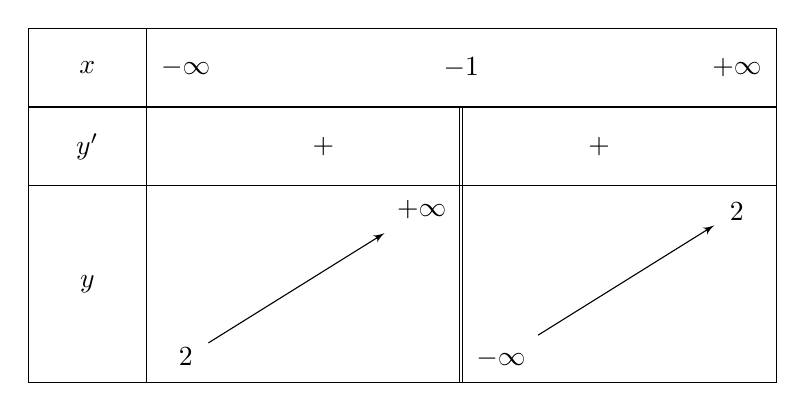
\begin{tikzpicture}
    \tkzTabInit[lgt=1.5, espcl=3.5]
    {$x$ /1, $y'$ /1, $y$ /2.5}
    {$-\infty$, $-1$, $+\infty$}
    \tkzTabLine{, +, d, +, }
    \tkzTabVar{-/ $2$ / , +D-/ $+\infty$ / $-\infty$, +/ $2$ /}
\end{tikzpicture}
\end{center}

Số giá trị nguyên của \( b \in [-2; 3] \) bằng}{
    \begin{tasks}(4)
        \task $6$
        \task $10$
        \task $4$
        \task $5$
    \end{tasks}
}

% --- CÂU 2 ---
\questionLinesManual{8}{2}{Cho hàm số \( f(x) = \dfrac{ax - 6}{bx + c} \) (\(a, b, c \in \mathbb{R}\)) có bảng biến thiên như sau:

\begin{center}
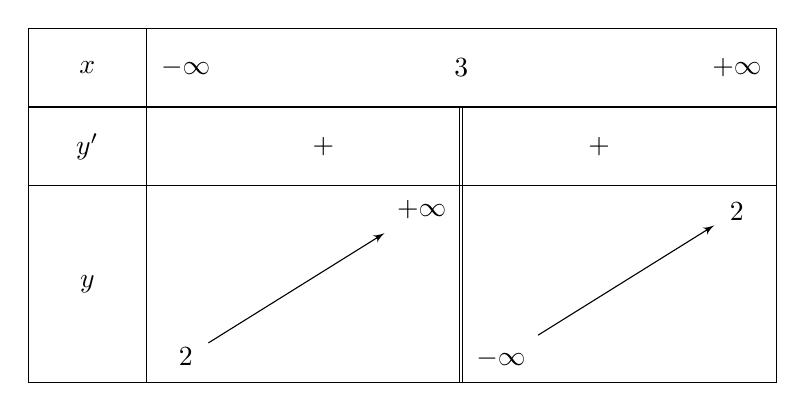
\begin{tikzpicture}
    \tkzTabInit[lgt=1.5, espcl=3.5]
    {$x$ /1, $y'$ /1, $y$ /2.5}
    {$-\infty$, $3$, $+\infty$}
    \tkzTabLine{, +, d, +, }
    \tkzTabVar{-/ $2$ / , +D-/ $+\infty$ / $-\infty$, +/ $2$ /}
\end{tikzpicture}
\end{center}

Giá trị nhỏ nhất của \( P = ab + a + c \) bằng:}{
    \begin{tasks}(4)
        \task $-\dfrac{1}{4}$
        \task $-\dfrac{3}{8}$
        \task $-\dfrac{25}{8}$
        \task $-\dfrac{1}{8}$
    \end{tasks}
}
% --- CÂU 3 ---
\questionLinesManual{8}{3}{Cho hàm số \( f(x) = \dfrac{mx^2 + nx + p}{qx + r} \) có bảng biến thiên như hình vẽ bên dưới

\begin{center}
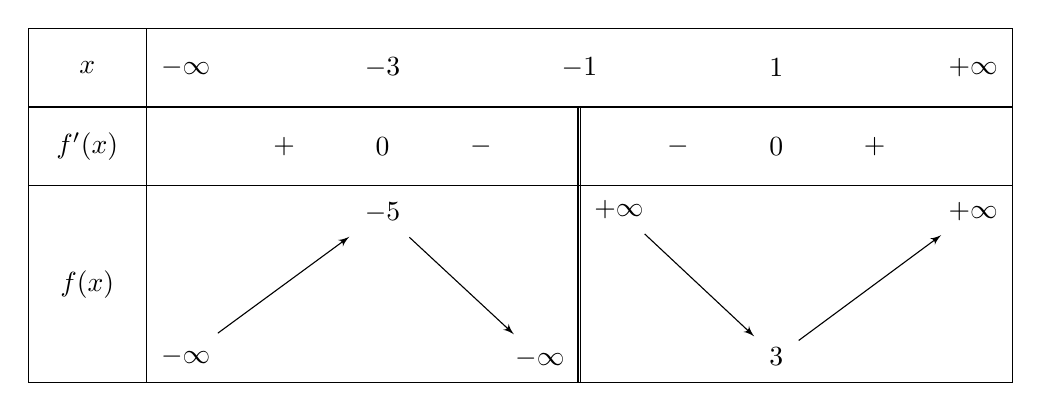
\begin{tikzpicture}
    \tkzTabInit[lgt=1.5, espcl=2.5]
    {$x$ /1, $f'(x)$ /1, $f(x)$ /2.5}
    {$-\infty$, $-3$, $-1$, $1$, $+\infty$}
    \tkzTabLine{, +, 0, -, d, -, 0, +, }
    \tkzTabVar{-/ $-\infty$ / , +/ $-5$ / , -D+/ $-\infty$ / $+\infty$ , -/ $3$ / , +/ $+\infty$ /}
\end{tikzpicture}
\end{center}

\( I \) là tâm đối xứng của đồ thị hàm số \( y = f(x) \). Tìm toạ độ \( I \).}{
    \begin{tasks}(4)
        \task \( I(-2;1) \)
        \task \( I(-1;1) \)
        \task \( I(-1;0) \)
        \task \( I(-1;-1) \)
    \end{tasks}
}

% --- CÂU 4 ---
\questionLinesManual{3}{4}{Cho hàm số \( y = f(x) \) xác định trên \( \mathbb{R} \setminus \{1\} \), liên tục trên mỗi khoảng xác định và có bảng biến thiên hình vẽ sau

\begin{center}
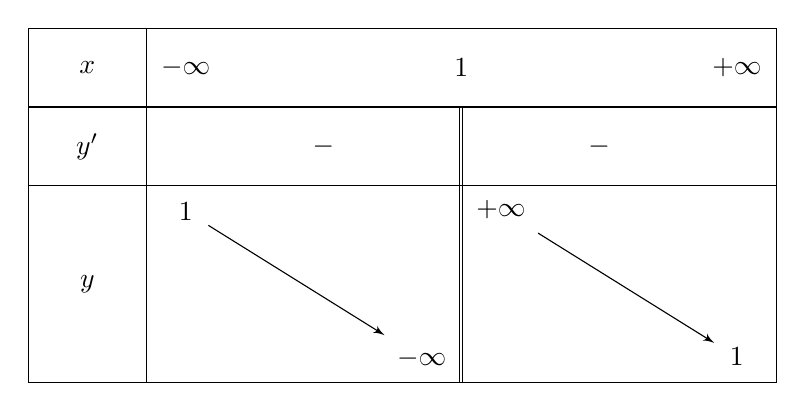
\begin{tikzpicture}
    \tkzTabInit[lgt=1.5, espcl=3.5]
    {$x$ /1, $y'$ /1, $y$ /2.5}
    {$-\infty$, $1$, $+\infty$}
    \tkzTabLine{, -, d, -, }
    \tkzTabVar{+/ $1$ / , -D+/ $-\infty$ / $+\infty$ , -/ $1$ /}
\end{tikzpicture}
\end{center}

Bảng biến thiên trên là của hàm số nào trong các hàm số sau?}{
    \begin{tasks}(4)
        \task \( y = \dfrac{-x+2}{x-1} \)
        \task \( y = \dfrac{x+2}{x-1} \)
        \task \( y = \dfrac{x-3}{x-1} \)
        \task \( y = \dfrac{x+2}{x+1} \)
    \end{tasks}
}

% --- CÂU 5 ---
\questionLinesManual{3}{5}{Cho hàm số \( f(x) = \dfrac{ax^2 + bx + c}{ex + f} \) có bảng biến thiên như hình sau:

\begin{center}
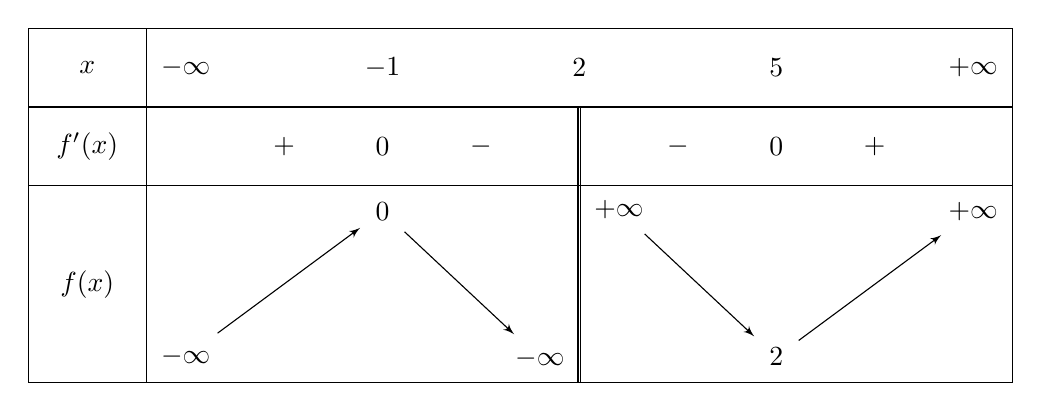
\begin{tikzpicture}
    \tkzTabInit[lgt=1.5, espcl=2.5]
    {$x$ /1, $f'(x)$ /1, $f(x)$ /2.5}
    {$-\infty$, $-1$, $2$, $5$, $+\infty$}
    \tkzTabLine{, +, 0, -, d, -, 0, +, }
    \tkzTabVar{-/ $-\infty$ / , +/ $0$ / , -D+/ $-\infty$ / $+\infty$ , -/ $2$ / , +/ $+\infty$ /}
\end{tikzpicture}
\end{center}

Hàm số đã cho đạt cực đại tại điểm}{
    \begin{tasks}(4)
        \task \( x = 5 \)
        \task \( x = 2 \)
        \task \( x = 0 \)
        \task \( x = -1 \)
    \end{tasks}
}
% --- CÂU 6 ---
\questionLinesManual{3}{6}{Đường cong trong hình vẽ bên là của đồ thị hàm số nào trong các hàm số được cho bởi các phương án A, B, C, D dưới đây?

\begin{center}
\begin{tikzpicture}[>=latex, scale=0.8]
    % 2. Vẽ hệ trục tọa độ
    \draw[->] (-3.5,0) -- (5,0) node[below] {\small$x$};
    \draw[->] (0,-3.5) -- (0,5) node[right] {\small $y$};
    \node[below left] at (0,0) {\small $O$};
    % 4. Vẽ đồ thị hàm số y = (2x-1)/(x-1)
    \draw[thick, samples=100, domain=-3.5:0.55] 
        plot (\x, {(\x + 1)/(\x - 1)});
    \draw[thick, samples=100, domain=1.5:5] 
        plot (\x, {(\x + 1)/(\x - 1)});
    
    % 5. Đường tiệm cận
    \draw[thick] (1,-3.5) -- (1,5) ;
    \draw[thick] (-3.5,1) -- (5,1) ;
    \node [below right] at (1,0) {\small$1$};
    \node [below left] at (0,1) {\small $1$};
    
\end{tikzpicture}
\end{center}

}{
    \begin{tasks}(4)
        \task \( y = \dfrac{2x - 1}{x - 1} \)
        \task \( y = \dfrac{-x + 1}{x + 1} \)
        \task \( y = \dfrac{2x - 2}{2x + 1} \)
        \task \( y = \dfrac{x + 1}{x - 1} \)
    \end{tasks}
}

% --- CÂU 7 ---
\questionLinesManual{3}{7}{Cho hàm số \( y = \dfrac{ax + b}{cx + d} \) có đồ thị là đường cong như hình vẽ bên. Tọa độ tâm đối xứng của đồ thị hàm số đã cho là

\begin{center}
\begin{tikzpicture}[>=latex, scale=0.8]

    \draw[->] (-3.5,0) -- (5.5,0) node[below] {\small $x$};
    \draw[->] (0,-3.5) -- (0,5.5) node[right] {\small $y$};
    \node[below left] at (0,0) {\small $O$};
    % Vẽ đồ thị hàm số y = (x+1)/(x-1)
    \draw[thick, samples=100, domain=-3.5:0.65] 
        plot (\x, {(0.5*\x + 1)/(\x - 1)});
    \draw[thick, samples=100, domain=1.3:5.5] 
        plot (\x, {(0.5*\x + 1)/(\x - 1)});
    \node [below right] at (1,0) {\small$1$};
    \node [above left] at ( 0,0.5) {\small$\dfrac{1}{2}$};
    % Đường tiệm cận
    \draw[thick] (1,-3.5) -- (1,5.5);
    \draw[thick] (-3.5,0.5) -- (5.5,0.5);
    
\end{tikzpicture}
\end{center}

}{
    \begin{tasks}(4)
        \task \( \left( 0; \dfrac{1}{2} \right) \)
        \task \( (1; 0) \)
        \task \( \left( \dfrac{1}{2}; 1 \right) \)
        \task \( (1; 1) \)
    \end{tasks}
}

% --- CÂU 8 ---
\questionLinesManual{3}{8}{Cho hàm số \( y = \dfrac{ax + b}{cx + d} \) có đồ thị là đường cong như hình vẽ bên. Tọa độ giao điểm của đồ thị hàm số với trục hoành là

\begin{center}
\begin{tikzpicture}[>=latex, scale=0.8]
    % Hệ trục tọa độ
    \draw[->] (-3.5,0) -- (5.5,0) node[below] {\small $x$};
    \draw[->] (0,-3.5) -- (0,5.5) node[right] {\small $y$};
    \node[below left] at (0,0) {\small $O$};
    
    % Đánh dấu các mốc
    \foreach \x in {1,2} {
        \draw (\x,0.05) -- (\x,-0.05) node[below right] {\small $\x$};
    }
    \foreach \val in {1,2} {
        \draw (0.05,\val) -- (-0.05,\val) node[ above left] {\small$\val$};
    }
    
    % Vẽ đồ thị hàm số y = (x+1)/(x-1)
    \draw[thick, samples=100, domain=-3.5:0.77] 
        plot (\x, {(\x -2)/(\x - 1)});
    \draw[thick, samples=100, domain=1.23:5.5] 
        plot (\x, {(\x -2)/(\x - 1)});
    
    % Đường tiệm cận
    \draw[thick] (1,-3.5) -- (1,5.5) ;
    \draw[thick] (-3.5,1) -- (5.5,1) ;
    
\end{tikzpicture}
\end{center}

}{
    \begin{tasks}(4)
        \task \( (0; 2) \)
        \task \( (0; 1) \)
        \task \( (1; 0) \)
        \task \( (2; 0) \)
    \end{tasks}
}

% --- CÂU 9 ---
\questionLinesManual{3}{9}{Hàm số nào dưới đây có đồ thị như hình vẽ sau?

\begin{center}
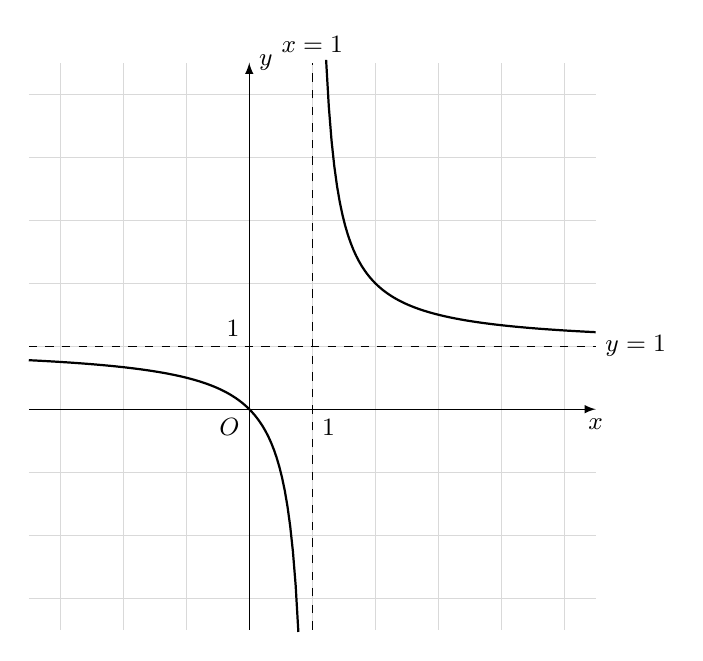
\begin{tikzpicture}[>=latex, scale=0.8]
    % 1. Vẽ lưới
    \draw[color=gray!30, thin, step=1] (-3.5,-3.5) grid (5.5,5.5);
    
    % 2. Vẽ hệ trục tọa độ
    \draw[->] (-3.5,0) -- (5.5,0) node[below] {\small $x$};
    \draw[->] (0,-3.5) -- (0,5.5) node[right] {\small $y$};
    \node[below left] at (0,0) {\small $O$};
    
    % 4. Vẽ đồ thị hàm số y = x/(x-1)
    \draw[thick, samples=100, domain=-3.5:0.78] 
        plot (\x, {\x/(\x - 1)});
    \draw[thick, samples=100, domain=1.22:5.5] 
        plot (\x, {\x/(\x - 1)});
    
    % 5. Đường tiệm cận
    \draw[dashed] (1,-3.5) -- (1,5.5) node[above] {\small $x=1$};
    \draw[dashed] (-3.5,1) -- (5.5,1) node[right] {\small $y=1$};
    \node[below right] at ( 1,0) {\small $1$};
    \node [ above left] at (0,1) {\small $1$};
\end{tikzpicture}
\end{center}

}{
    \begin{tasks}(4)
        \task \( y = \dfrac{x}{x+1} \)
        \task \( y = -\dfrac{x}{x-1} \)
        \task \( y = -\dfrac{x}{x+1} \)
        \task \( y = \dfrac{x}{x-1} \)
    \end{tasks}
}

% --- CÂU 10 ---
\questionLinesManual{3}{10}{Đường cong ở hình dưới đây là đồ thị của hàm số

\begin{center}
\begin{tikzpicture}[>=latex, scale=0.6]
    \draw[->] (-3.5,0) -- (4.5,0) node[below] {\small $x$};
    \draw[->] (0,-3.5) -- (0,5.5) node[right] {\small $y$};
    \node[below right] at (0,0) {\tiny $O$};
    
    % 3. Đánh dấu các mốc
    \foreach \x in {-3,-2,1,2,3,4} {
        \draw (\x,0.05) -- (\x,-0.05) node[below] {\tiny $\x$};
    }
    \foreach \val in {-3,-2,-1,1,2,3} {
        \draw (0.05,\val) -- (-0.05,\val) node[left] {\tiny $\val$};
    }
    
    % 4. Vẽ đồ thị hàm số y = (x^2 - x + 1)/(x - 1)
    \draw[thick, samples=100, domain=-3.5:0.76] 
        plot (\x, {(\x*\x - \x + 1)/(\x - 1)});
    \draw[thick, samples=100, domain=1.23:5.5] 
        plot (\x, {(\x*\x - \x + 1)/(\x - 1)});
    
    % 5. Đường tiệm cận
    \draw[dashed] (1,5.5) -- (1,-3.5) node[below] {\small $x=1$};
    \draw[dashed] (-3.5,-3.5) -- (5.5,5.5) node[ below right] {\small $y=x$};
\end{tikzpicture}
\end{center}

}{
    \begin{tasks}(4)
        \task \( y = \dfrac{x^2 - 4x + 5}{x - 2} \)
        \task \( y = \dfrac{x^2 - 4x - 1}{x + 1} \)
        \task \( y = \dfrac{x^2 - x + 1}{x - 1} \)
        \task \( y = \dfrac{x^2 + x - 1}{x - 1} \)
    \end{tasks}
}

% --- CÂU 11 ---
\questionLinesManual{5}{11}{Cho hàm số \( y = \dfrac{ax + b}{x + c} \) có đồ thị như hình sau đây

\begin{center}
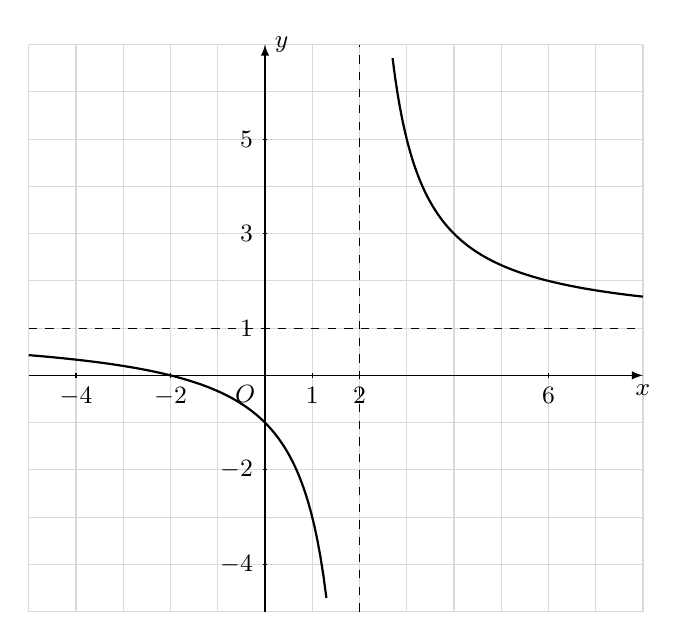
\begin{tikzpicture}[>=latex, scale=0.6]
    % 1. Vẽ lưới
    \draw[color=gray!30, thin, step=1] (-5,-5) grid (8,7);
    
    % 2. Vẽ hệ trục tọa độ
    \draw[->] (-5,0) -- (8,0) node[below] {\small $x$};
    \draw[->] (0,-5) -- (0,7) node[right] {\small $y$};
    \node[below left] at (0,0) {\small $O$};
    
    % 3. Đánh dấu các mốc
    \foreach \x in {-4,-2,1,2,6} {
        \draw (\x,0.05) -- (\x,-0.05) node[below] {\small $\x$};
    }
    \foreach \val in {-4,-2,1,3,5} {
        \draw (0.05,\val) -- (-0.05,\val) node[left] {\small $\val$};
    }
    
    % 4. Vẽ đồ thị hàm số y = (2x+1)/(x+1)
    \draw[thick, samples=100, domain=-5:1.3] 
        plot (\x, {(\x + 2)/(\x -2)});
    \draw[thick, samples=100, domain=2.7:8] 
        plot (\x, {(\x + 2)/(\x - 2)});
    
    % 5. Đường tiệm cận
    \draw[dashed] (2,-5) -- (2,7);
    \draw[dashed] (-5,1) -- (8,1);
\end{tikzpicture}
\end{center}

Tính giá trị của biểu thức \( P = 2a - b + 3c \).}{
    \begin{tasks}(4)
        \task $6$
        \task $-6$
        \task $10$
        \task $-2$
    \end{tasks}
}
% --- CÂU 12 ---
\questionLinesManual{5}{12}{Cho hàm số \( y = \dfrac{ax^2 + bx + 1}{cx + 2} \) (với \( a, b, c \in \mathbb{R}, a \neq 0 \)) có đồ thị là đường cong trong hình vẽ bên. Giá trị biểu thức \( T = 2a + 3b - c \) là

\begin{center}
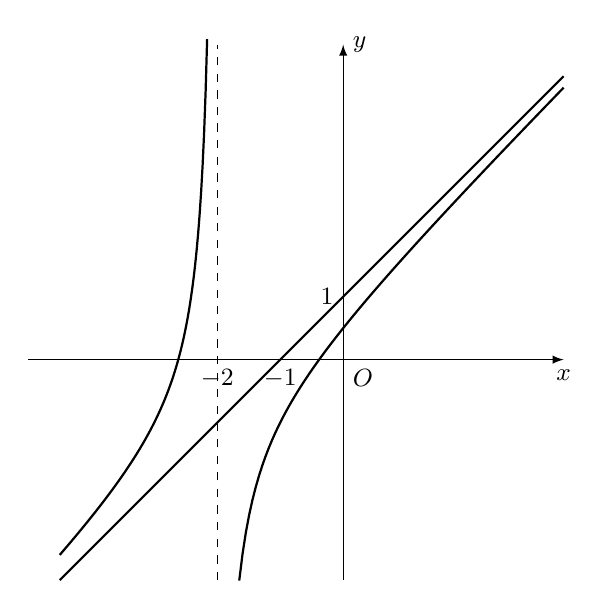
\begin{tikzpicture}[>=latex, scale=0.8]
    % 1. Hệ trục tọa độ
    \draw[->] (-5,0) -- (3.5,0) node[below] {\small $x$};
    \draw[->] (0,-3.5) -- (0,5) node[right] {\small $y$};
    \node[below right] at (0,0) {\small $O$};
    
    
    % 3. Vẽ đồ thị hàm số
    \draw[thick, samples=100, domain=-4.5:-2.16] 
        plot (\x, {\x+1 - 1/(\x + 2)});
    \draw[thick, samples=100, domain=-1.65:3.5] 
        plot (\x, {\x+1 - 1/(\x + 2)});
    \draw[thick, samples=100, domain=-4.5:3.5] 
        plot (\x, {\x+1 });
    % 4. Đường tiệm cận
    \draw[dashed] (-2,-3.5) -- (-2,5);
    \node [below] at (-2,0) {\small $-2$};
    \node [below] at (-1,0) {\small $-1$};
    \node [left] at (0,1) {\small $1$};
\end{tikzpicture}
\end{center}

}{
    \begin{tasks}(4)
        \task \( T = 11 \)
        \task \( T = 8 \)
        \task \( T = 9 \)
        \task \( T = 10 \)
    \end{tasks}
}

% --- CÂU 13 ---
\questionLinesManual{5}{13}{Cho hàm số \( y = ax + 2 + \dfrac{b}{x + c} \) có đồ thị như hình dưới đây. Giá trị của \( P = a + b + c \) bằng

\begin{center}
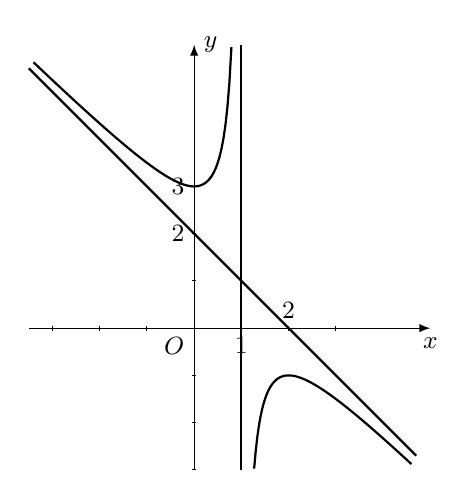
\begin{tikzpicture}[>=latex, scale=0.6]
    % 1. Hệ trục tọa độ
    \draw[->] (-3.5,0) -- (5,0) node[below] {\small $x$};
    \draw[->] (0,-3) -- (0,6) node[right] {\small $y$};
    \node[below left] at (0,0) {\small $O$};
    
    % 2. Đánh dấu các mốc
    \foreach \x in {-3,-2,-1,1,2,3} {
        \draw (\x,0.05) -- (\x,-0.05);
    }
    \foreach \val in {-3,-2,-1,1,2,3} {
        \draw (0.05,\val) -- (-0.05,\val) ;
    }
    
    % 3. Vẽ đồ thị hàm số
    \draw[thick, samples=100, domain=-3.4:0.79] 
        plot (\x, {-\x + 2 -1/(\x - 1)});
    \draw[thick, samples=100, domain=1.27:4.6] 
        plot (\x, {-\x + 2 -1/(\x - 1)});
    \draw[thick, samples=100, domain=-3.5:4.7] 
        plot (\x, {-\x + 2 });
    \node[below] at (1,0) {\small $1$};
    \node[above] at (2,0) {\small $2$};
    \node[left] at (0,2) {\small $2$};
    \node[left] at (0,3) {\small $3$};
    % 4. Đường tiệm cận
    \draw[thick] (1,-3) -- (1,6);
\end{tikzpicture}
\end{center}

}{
    \begin{tasks}(4)
        \task $1$
        \task $-1$
        \task $2$
        \task $-3$
    \end{tasks}
}

% --- CÂU 14 ---
\questionLinesManual{3}{14}{Đường cong trong hình vẽ sau là đồ thị của hàm số nào dưới đây?

\begin{center}
\begin{tikzpicture}[>=latex, scale=0.8]
    % 1. Hệ trục tọa độ
    \draw[->] (-3.5,0) -- (5.5,0) node[below] {\small $x$};
    \draw[->] (0,-3.5) -- (0,3.5) node[right] {\small $y$};
    \node[below right] at (0,0) {\small $O$};
    
    
    % 3. Vẽ đồ thị hàm số y = (x+1)/(x-1)
    \draw[thick, samples=100, domain=-3.5:0.55] 
        plot (\x, {(\x + 1)/(\x - 1)});
    \draw[thick, samples=100, domain=1.78:5.5] 
        plot (\x, {(\x + 1)/(\x - 1)});
    
    % 4. Đường tiệm cận
    \draw[dashed] (1,-3.5) -- (1,3.5);
    \draw[dashed] (-3.5,1) -- (5.5,1) ;
    \node[below] at (-1,0) {\small $-1$};
    \node[below] at (1,0) {\small $1$};
    \node[left] at (0,-1) {\small $-1$};
    \node[left] at (0,1) {\small $1$};
\end{tikzpicture}
\end{center}

}{
    \begin{tasks}(4)
        \task \( y = \dfrac{x^2 - x + 1}{x - 1} \)
        \task \( y = \dfrac{2x - 1}{x - 1} \)
        \task \( y = \dfrac{x + 1}{x - 1} \)
        \task \( y = x^3 - 3x - 1 \)
    \end{tasks}
}

% --- CÂU 15 ---
\questionLinesManual{3}{15}{Đường cong trong hình vẽ là đồ thị của hàm số nào dưới đây?

\begin{center}
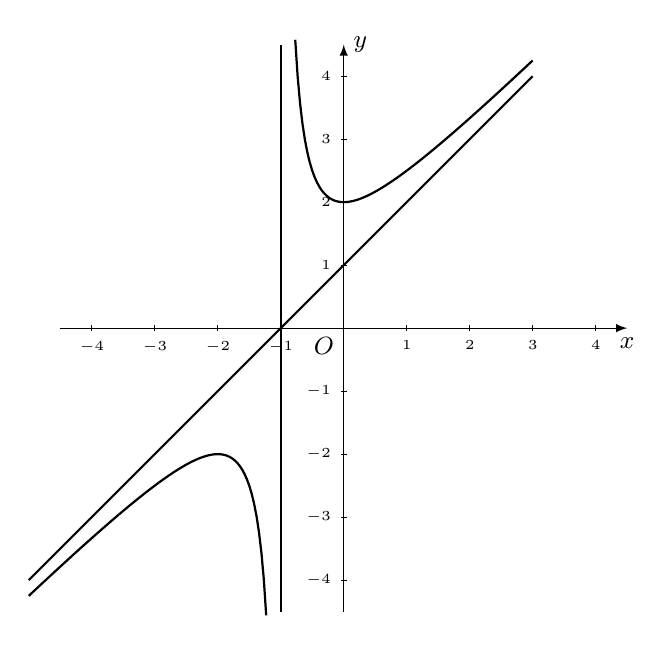
\begin{tikzpicture}[>=latex, scale=0.8]
    % 1. Hệ trục tọa độ
    \draw[->] (-4.5,0) -- (4.5,0) node[below] {\small $x$};
    \draw[->] (0,-4.5) -- (0,4.5) node[right] {\small $y$};
    \node[below left] at (0,0) {\small $O$};
    
    % 2. Đánh dấu các mốc
    \foreach \x in {-4,-3,-2,-1,1,2,3,4} {
        \draw (\x,0.05) -- (\x,-0.05) node[below] {\tiny $\x$};
    }
    \foreach \val in {-4,-3,-2,-1,1,2,3,4} {
        \draw (0.05,\val) -- (-0.05,\val) node[left] {\tiny $\val$};
    }
    
    % 3. Vẽ đồ thị hàm số y = (x^2 + 2x + 2)/(x + 1)
    \draw[thick, samples=100, domain=-5:-1.23] 
        plot (\x, {(\x*\x + 2*\x + 2)/(\x + 1)});
    \draw[thick, samples=100, domain=-0.77:3] 
        plot (\x, {(\x*\x + 2*\x + 2)/(\x + 1)});
    \draw[thick, samples=100, domain=-5:3] 
        plot (\x, {\x+1});
    
    % 4. Đường tiệm cận
    \draw[thick] (-1,-4.5) -- (-1,4.5);
\end{tikzpicture}
\end{center}

}{
    \begin{tasks}(4)
        \task \( y = \dfrac{x^2 + 2x + 2}{x + 1} \)
        \task \( y = \dfrac{x^2 - 2x - 3}{x - 2} \)
        \task \( y = \dfrac{x^2 + 3x}{x - 2} \)
        \task \( y = \dfrac{x^2 - 2x}{x + 1} \)
    \end{tasks}
}

% --- CÂU 16 ---
\questionLinesManual{3}{16}{Đường cong ở dưới đây là đồ thị của hàm số nào?

\begin{center}
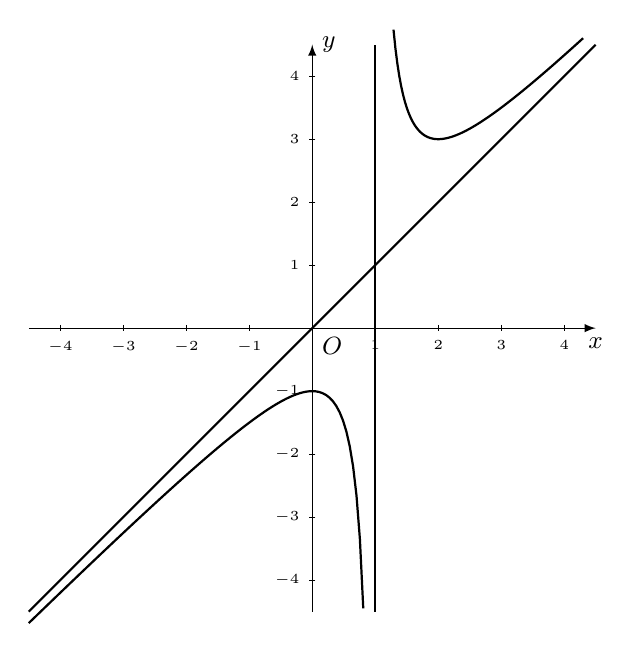
\begin{tikzpicture}[>=latex, scale=0.8]
    % 1. Hệ trục tọa độ
    \draw[->] (-4.5,0) -- (4.5,0) node[below] {\small $x$};
    \draw[->] (0,-4.5) -- (0,4.5) node[right] {\small $y$};
    \node[below right] at (0,0) {\small $O$};
    
    % 2. Đánh dấu các mốc
    \foreach \x in {-4,-3,-2,-1,1,2,3,4} {
        \draw (\x,0.05) -- (\x,-0.05) node[below] {\tiny $\x$};
    }
    \foreach \val in {-4,-3,-2,-1,1,2,3,4} {
        \draw (0.05,\val) -- (-0.05,\val) node[left] {\tiny $\val$};
    }
    
    % 3. Vẽ đồ thị hàm số y = (x^2 + x - 1)/(x - 1)
    \draw[thick, samples=100, domain=-4.5:0.81] 
        plot (\x, {(\x*\x - \x + 1)/(\x - 1)});
    \draw[thick, samples=100, domain=1.29:4.3] 
        plot (\x, {(\x*\x - \x +1)/(\x - 1)});
    \draw[thick, samples=100, domain=-4.5:4.5] 
        plot (\x, {(\x});
    % 4. Đường tiệm cận
    \draw[thick] (1,-4.5) -- (1,4.5) ;
    
\end{tikzpicture}
\end{center}

}{
    \begin{tasks}(4)
        \task \( y = \dfrac{x^2 + x - 1}{x - 1} \)
        \task \( y = \dfrac{x^2 - x + 1}{x - 1} \)
        \task \( y = \dfrac{x^2 - 4x - 1}{x + 1} \)
        \task \( y = \dfrac{x^2 - 4x + 5}{x - 2} \)
    \end{tasks}
}

% --- CÂU 17 ---
\questionLinesManual{3}{17}{Đồ thị của hàm số \( y = \dfrac{x+1}{-x+1} \) là đường cong nào trong các hình vẽ sau?

\begin{center}

\end{center}

}{
    \begin{tasks}(2)
        \task \(
        \begin{tikzpicture}[>=latex, scale=0.8]
                % 1. Hệ trục tọa độ
                \draw[->] (-4.5,0) -- (3.5,0) node[below] {\small $x$};
                \draw[->] (0,-3.5) -- (0,4.5) node[right] {\small $y$};
                \node[below left] at (0,0) {\small $O$};
                
                % 2. Đánh dấu các mốc
                \foreach \x in {-1,1} {
                    \draw (\x,0.05) -- (\x,-0.05) node[below] {\small $\x$};
                }
                \foreach \val in {1} {
                    \draw (0.05,\val) -- (-0.05,\val) node[left] {\small $\val$};
                }
                
                % 3. Vẽ đồ thị hàm số y = (x+1)/(-x+1) = -(x+1)/(x-1)
                \draw[thick, samples=100, domain=-4.5:-1.57] 
                    plot (\x, {(\x - 1)/(\x + 1)});
                \draw[thick, samples=100, domain=-0.57:3.5] 
                    plot (\x, {(\x - 1)/(\x + 1)});
                
                % 4. Đường tiệm cận
                \draw[dashed] (-1,-3.5) -- (-1,4.5) ;
                \draw[dashed] (-4.5,1) -- (3.5,1) ;
            \end{tikzpicture}
        \)
        
        \task \(
        \begin{tikzpicture}[>=latex, scale=0.8]
                % 1. Hệ trục tọa độ
                \draw[->] (-3.5,0) -- (4.5,0) node[below] {\small $x$};
                \draw[->] (0,-4.5) -- (0,3.5) node[right] {\small $y$};
                \node[below left] at (0,0) {\small $O$};
                
                % 2. Đánh dấu các mốc
                \foreach \x in {-1,1} {
                    \draw (\x,0.05) -- (\x,-0.05) node[below] {\small $\x$};
                }
                \foreach \val in {-1,1} {
                    \draw (0.05,\val) -- (-0.05,\val) node[left] {\small $\val$};
                }
                
                % 3. Vẽ đồ thị hàm số y = (x+1)/(-x+1) = -(x+1)/(x-1)
                \draw[thick, samples=100, domain=-3.5:0.56] 
                    plot (\x, {(\x + 1)/(-\x + 1)});
                \draw[thick, samples=100, domain=1.57:4.5] 
                    plot (\x, {(\x + 1)/(-\x + 1)});
                
                % 4. Đường tiệm cận
                \draw[dashed] (1,-4.5) -- (1,3.5) ;
                \draw[dashed] (-3.5,-1) -- (4.5,-1) ;
            \end{tikzpicture}
        \)
        \task \(
        \begin{tikzpicture}[>=latex, scale=0.8]
                % 1. Hệ trục tọa độ
                \draw[->] (-4.5,0) -- (3.5,0) node[below] {\small $x$};
                \draw[->] (0,-4.5) -- (0,3.5) node[right] {\small $y$};
                \node[below left] at (0,0) {\small $O$};
                
                % 2. Đánh dấu các mốc
                \foreach \x in {-1,1} {
                    \draw (\x,0.05) -- (\x,-0.05) node[below] {\small $\x$};
                }
                \foreach \val in {-1,1} {
                    \draw (0.05,\val) -- (-0.05,\val) node[below left] {\small $\val$};
                }
                
                % 3. Vẽ đồ thị hàm số y = (x+1)/(-x+1) = -(x+1)/(x-1)
                \draw[thick, samples=100, domain=-4.5:-1.57] 
                    plot (\x, {(\x - 1)/(-\x - 1)});
                \draw[thick, samples=100, domain=-0.56:3.5] 
                    plot (\x, {(\x - 1)/(-\x - 1)});
                
                % 4. Đường tiệm cận
                \draw[dashed] (-1,-4.5) -- (-1,3.5);
                \draw[dashed] (-4.5,-1) -- (3.5,-1);
            \end{tikzpicture}
        \)
        \task \(
        \begin{tikzpicture}[>=latex, scale=0.8]
                % 1. Hệ trục tọa độ
                \draw[->] (-3.5,0) -- (4.5,0) node[below] {\small $x$};
                \draw[->] (0,-3.5) -- (0,4.5) node[right] {\small $y$};
                \node[below left] at (0,0) {\small $O$};
                
                % 2. Đánh dấu các mốc
                \foreach \x in {-1,1} {
                    \draw (\x,0.05) -- (\x,-0.05) node[below] {\small $\x$};
                }
                \foreach \val in {-1,1} {
                    \draw (0.05,\val) -- (-0.05,\val) node[left] {\small $\val$};
                }
                
                % 3. Vẽ đồ thị hàm số y = (x+1)/(-x+1) = -(x+1)/(x-1)
                \draw[thick, samples=100, domain=-3.5:0.56] 
                    plot (\x, {(\x + 1)/(\x - 1)});
                \draw[thick, samples=100, domain=1.57:4.5] 
                    plot (\x, {(\x + 1)/(\x - 1)});
                
                % 4. Đường tiệm cận
                \draw[dashed] (1,-3.5) -- (1,4.5) ;
                \draw[dashed] (-3.5,1) -- (4.5,1);
            \end{tikzpicture}
        \)
    \end{tasks}
}

% --- CÂU 18 ---
\questionLinesManual{3}{18}{Cho hàm số \( y = \dfrac{ax + b}{cx + d} \) (\(a, b, c \in \mathbb{R}\)) có đồ thị là đường cong như hình vẽ bên:

\begin{center}
\begin{tikzpicture}[>=latex, scale=0.8]
    % 1. Hệ trục tọa độ
    \draw[->] (-4.5,0) -- (3.5,0) node[below] {\small $x$};
    \draw[->] (0,-3.5) -- (0,4.5) node[right] {\small $y$};
    \node[below left] at (0,0) {\small $O$};
    % 3. Vẽ đồ thị hàm số y = (x+1)/(x-1)
    \draw[thick, samples=100, domain=-4.5:-1.56] 
        plot (\x, {(\x - 1)/(\x + 1)});
    \draw[thick, samples=100, domain=-0.56:3.5] 
        plot (\x, {(\x - 1)/(\x +1)});
    
    % 4. Đường tiệm cận
    \draw[dashed] (-1,-3.5) -- (-1,4.5);
    \draw[dashed] (-4.5,1) -- (3.5,1);
    
    \node[below left] at (-1,0) {\small $-1$};
    \node [above left] at ( 0,1) {\small $1$};
\end{tikzpicture}
\end{center}

Toạ độ tâm đối xứng của đồ thị hàm số đã cho là:}{
    \begin{tasks}(4)
        \task \((-1; 1)\)
        \task \((1; 1)\)
        \task \((1; -1)\)
        \task \((0; 1)\)
    \end{tasks}
}

% --- CÂU 19 ---
\questionLinesManual{3}{19}{Cho hàm số \( y = f(x) \) có đồ thị như hình dưới đây. Biểu thức \( f(x) \) là biểu thức nào sau đây?

\begin{center}
\begin{tikzpicture}[>=latex, scale=0.8]
    % 1. Hệ trục tọa độ
    \draw[->] (-4.5,0) -- (3.5,0) node[below] {\small $x$};
    \draw[->] (0,-3.5) -- (0,4.5) node[right] {\small $y$};
    \node[below left] at (0,0) {\small $O$};
    % 3. Vẽ đồ thị hàm số y = (x+1)/(x-1)
    \draw[thick, samples=100, domain=-4.5:-1.56] 
        plot (\x, {(\x - 1)/(\x + 1)});
    \draw[thick, samples=100, domain=-0.56:3.5] 
        plot (\x, {(\x - 1)/(\x +1)});
    
    % 4. Đường tiệm cận
    \draw[dashed] (-1,-3.5) -- (-1,4.5);
    \draw[dashed] (-4.5,1) -- (3.5,1);
    
    
    \node[below left] at (-1,0) {\small $-1$};
    \node [above left] at ( 0,1) {\small $1$};
\end{tikzpicture}
\end{center}

}{
    \begin{tasks}(4)
        \task \( x + \dfrac{1}{x} \)
        \task \( -x^3 + 3x - 1 \)
        \task \( x^3 - 1 \)
        \task \( \dfrac{x - 1}{x + 1} \)
    \end{tasks}
}


% --- CÂU 20 ---
\questionLinesManual{3}{20}{Cho hàm số \( y = \dfrac{ax + b}{cx + d} \) (với \( c \neq 0, ad - bc \neq 0 \)) có đồ thị như hình vẽ bên. Khẳng định nào sau đây đúng?

\begin{center}
\begin{tikzpicture}[>=latex, scale=0.8]
    % 1. Hệ trục tọa độ
    \draw[->] (-3.5,0) -- (4.5,0) node[below] {\small $x$};
    \draw[->] (0,-3.5) -- (0,4.5) node[right] {\small $y$};
    \node[below left] at (0,0) {\small $O$};
    
    % 2. Đánh dấu các mốc
    \foreach \x in {1,2} {
        \draw (\x,0.05) -- (\x,-0.05) node[below] {\small $\x$};
    }
    \foreach \val in {1,2} {
        \draw (0.05,\val) -- (-0.05,\val) node[left] {\small $\val$};
    }
    
    % 3. Vẽ đồ thị hàm số y = (x+2)/(x-1)
    \draw[thick, samples=100, domain=-3.5:0.7] 
        plot (\x, {(\x - 2)/(\x - 1)});
    \draw[thick, samples=100, domain=1.23:4.5] 
        plot (\x, {(\x - 2)/(\x - 1)});
    
    % 4. Đường tiệm cận
    \draw[dashed] (1,-3.5) -- (1,4.5);
    \draw[dashed] (-3.5,1) -- (4.5,1);
\end{tikzpicture}
\end{center}

}{
    \begin{tasks}(1)
        \task Đồ thị hàm số có hai điểm cực trị.
        \task \( \lim\limits_{x \to -\infty} f(x) = +\infty \) và \( \lim\limits_{x \to +\infty} f(x) = -\infty \).
        \task \( \lim\limits_{x \to 1^-} f(x) = -\infty \) và \( \lim\limits_{x \to 1^+} f(x) = +\infty \).
        \task Hàm số đồng biến trên khoảng \((-\infty; +\infty)\).
    \end{tasks}
}

% --- CÂU 21 ---
\questionLinesManual{3}{21}{Đường cong như hình vẽ dưới đây là đồ thị của hàm số nào?

\begin{center}
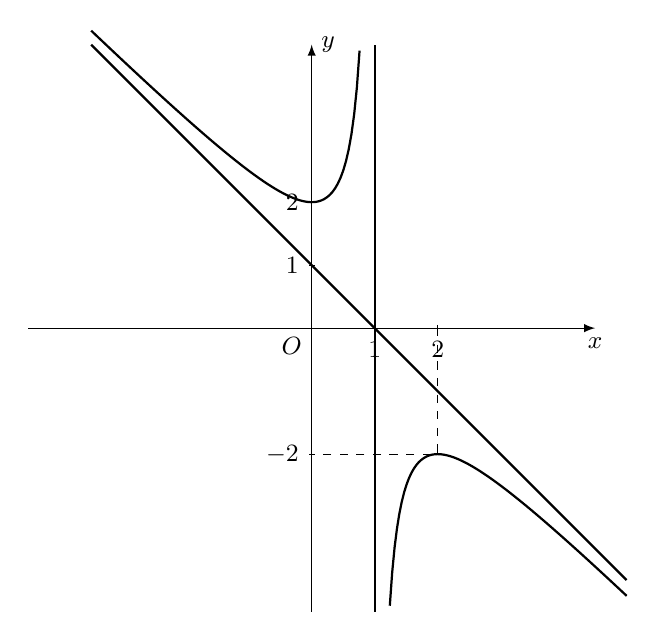
\begin{tikzpicture}[>=latex, scale=0.8]
    % 1. Hệ trục tọa độ
    \draw[->] (-4.5,0) -- (4.5,0) node[below] {\small $x$};
    \draw[->] (0,-4.5) -- (0,4.5) node[right] {\small $y$};
    \node[below left] at (0,0) {\small $O$};
    
    % 2. Đánh dấu các mốc
    \foreach \x in {1,2} {
        \draw (\x,0.05) -- (\x,-0.05) node[below] {\small $\x$};
    }
    \foreach \val in {-2,1,2} {
        \draw (0.05,\val) -- (-0.05,\val) node[left] {\small $\val$};
    }
    
    % 3. Vẽ đồ thị hàm số y = (-x^2 + 2x - 2)/(x-1)
    \draw[thick, samples=100, domain=-3.5:0.76] 
        plot (\x, {(-\x*\x + 2*\x - 2)/(\x - 1)});
    \draw[thick, samples=100, domain=1.24:5] 
        plot (\x, {(-\x*\x + 2*\x - 2)/(\x - 1)});
     \draw[thick, samples=100, domain=-3.5:5] 
        plot (\x, {(-\x+1});
    % 4. Đường tiệm cận
    \draw[thick] (1,-4.5) -- (1,4.5);
    \draw [dashed] (2,0) -- ( 2,-2) -- ( 0,-2);
\end{tikzpicture}
\end{center}

}{
    \begin{tasks}(4)
        \task \( y = \dfrac{x-2}{x-1} \)
        \task \( y = \dfrac{x^2 + 2x - 2}{x-1} \)
        \task \( y = \dfrac{-x^2 + 2x - 2}{x-1} \)
        \task \( y = \dfrac{-x^2 + x - 2}{x-1} \)
    \end{tasks}
}

% --- CÂU 22 ---
\questionLinesManual{3}{22}{Đồ thị trong hình vẽ dưới đây là của hàm số nào?

\begin{center}
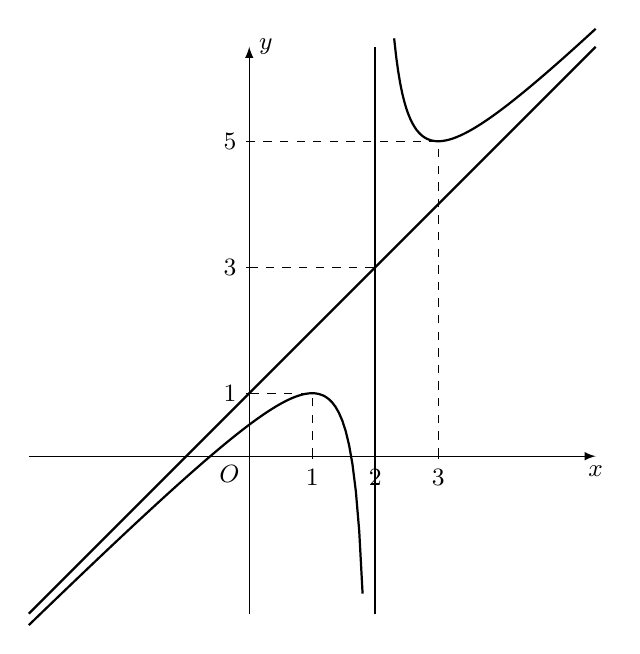
\begin{tikzpicture}[>=latex, scale=0.8]
    % 1. Hệ trục tọa độ
    \draw[->] (-3.5,0) -- (5.5,0) node[below] {\small $x$};
    \draw[->] (0,-2.5) -- (0,6.5) node[right] {\small $y$};
    \node[below left] at (0,0) {\small $O$};
    
    % 2. Đánh dấu các mốc
    \foreach \x in {1,2,3} {
        \draw (\x,0.05) -- (\x,-0.05) node[below] {\small $\x$};
    }
    \foreach \val in {1,5,3} {
        \draw (0.05,\val) -- (-0.05,\val) node[left] {\small $\val$};
    }
    
    % 3. Vẽ đồ thị hàm số y = (x^2 - x - 1)/(x - 1)
    \draw[thick, samples=100, domain=-3.5:1.8] 
        plot (\x, {(\x*\x - \x - 1)/(\x - 2)});
    \draw[thick, samples=100, domain=2.3:5.5] 
        plot (\x, {(\x*\x - \x - 1)/(\x - 2)});
     \draw[thick, samples=100, domain=-3.5:5.5] 
        plot (\x, {(\x+1});
    % 4. Đường tiệm cận
    \draw[thick] (2,-2.5) -- (2,6.5) ;
    \draw[dashed] (1,0) -- (1,1) -- (0,1);
    \draw[dashed] (0,3) -- ( 2,3);
    \draw[dashed] (3,0) -- (3,5) -- (0,5);
\end{tikzpicture}
\end{center}

}{
    \begin{tasks}(4)
        \task \( y = \dfrac{x^2 - x - 1}{x - 2} \)
        \task \( y = \dfrac{x - 2}{1 - 3x} \)
        \task \( y = \dfrac{x^2 - x - 1}{x - 1} \)
        \task \( y = -x^3 + 3x^2 + 1 \)
    \end{tasks}
}

% --- CÂU 23 ---
\questionLinesManual{3}{23}{Đường cong nào dưới đây là đồ thị của hàm số \( y = \dfrac{x+1}{x-1} \)?

}{
    \begin{tasks}(2)
        \task \(
        \begin{tikzpicture}[>=latex, scale=0.8]
            % 1. Hệ trục tọa độ
            \draw[->] (-4.5,0) -- (4.5,0) node[below] {\small $x$};
            \draw[->] (0,-4.5) -- (0,4.5) node[right] {\small $y$};
            \node[below left] at (0,0) {\tiny $O$};
            
            % 2. Đánh dấu các mốc
            \foreach \x in {-4,-3,-2,-1,1,2,3,4} {
                \draw (\x,0.05) -- (\x,-0.05) node[below] {\tiny $\x$};
            }
            \foreach \val in {-4,-3,-2,-1,1,2,3,4} {
                \draw (0.05,\val) -- (-0.05,\val) node[left] {\tiny$\val$};
            }
            
            % 3. Vẽ đồ thị hàm số y = (x+1)/(x-1)
            \draw[thick, samples=100, domain=-1.7:1.5] 
                plot (\x, {\x*\x*\x+1});
        \end{tikzpicture}
        \)
        \task \(
        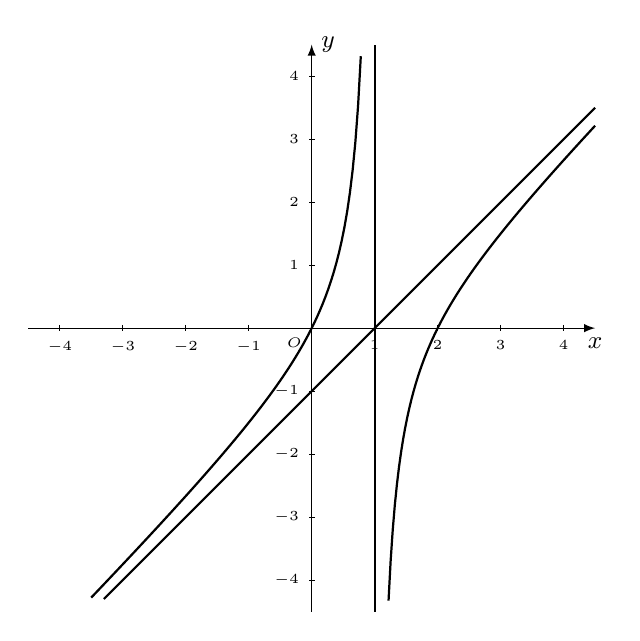
\begin{tikzpicture}[>=latex, scale=0.8]
            % 1. Hệ trục tọa độ
            \draw[->] (-4.5,0) -- (4.5,0) node[below] {\small $x$};
            \draw[->] (0,-4.5) -- (0,4.5) node[right] {\small $y$};
            \node[below left] at (0,0) {\tiny $O$};
            
            % 2. Đánh dấu các mốc
            \foreach \x in {-4,-3,-2,-1,1,2,3,4} {
                \draw (\x,0.05) -- (\x,-0.05) node[below] {\tiny $\x$};
            }
            \foreach \val in {-4,-3,-2,-1,1,2,3,4} {
                \draw (0.05,\val) -- (-0.05,\val) node[left] {\tiny$\val$};
            }
            
            \draw[thick, samples=100, domain=-3.5:0.78] 
                plot (\x, {\x-1 -1/(\x-1)});
            \draw[thick, samples=100, domain=1.22:4.5] 
                plot (\x, {\x-1 -1/(\x-1)});
            \draw[thick, samples=100, domain=-3.3:4.5]                      plot (\x, {\x-1});  
            
            % 4. Đường tiệm cận
            \draw[thick] (1,-4.5) -- (1,4.5);
        \end{tikzpicture}
        \)
        \task \(
        \begin{tikzpicture}[>=latex, scale=0.8]
            % 1. Hệ trục tọa độ
            \draw[->] (-4.5,0) -- (4.5,0) node[below] {\small $x$};
            \draw[->] (0,-4.5) -- (0,4.5) node[right] {\small $y$};
            \node[below left] at (0,0) {\tiny $O$};
            
            % 2. Đánh dấu các mốc
            \foreach \x in {-4,-3,-2,-1,1,2,3,4} {
                \draw (\x,0.05) -- (\x,-0.05) node[below] {\tiny $\x$};
            }
            \foreach \val in {-4,-3,-2,-1,1,2,3,4} {
                \draw (0.05,\val) -- (-0.05,\val) node[left] {\tiny$\val$};
            }
            % 3. Vẽ đồ thị hàm số y = (x+1)/(x-1)
            \draw[thick, samples=100, domain=-4.5:0.64] 
                plot (\x, {(\x + 1)/(\x - 1)});
            \draw[thick, samples=100, domain=1.56:4.5] 
                plot (\x, {(\x + 1)/(\x - 1)});
            
            % 4. Đường tiệm cận
            \draw[thick] (1,-4.5) -- (1,4.5);
            \draw[thick] (-4.5,1) -- (4.5,1);
        \end{tikzpicture}
        \)
        \task \(
        \begin{tikzpicture}[>=latex, scale=0.8]
            % 1. Hệ trục tọa độ
            \draw[->] (-4.5,0) -- (4.5,0) node[below] {\small $x$};
            \draw[->] (0,-4.5) -- (0,4.5) node[right] {\small $y$};
            \node[below left] at (0,0) {\tiny $O$};
            
            % 2. Đánh dấu các mốc
            \foreach \x in {-4,-3,-2,-1,1,2,3,4} {
                \draw (\x,0.05) -- (\x,-0.05) node[below] {\tiny $\x$};
            }
            \foreach \val in {-4,-3,-2,-1,1,2,3,4} {
                \draw (0.05,\val) -- (-0.05,\val) node[left] {\tiny$\val$};
            }
            % 3. Vẽ đồ thị hàm số y = (x+1)/(x-1)
            \draw[thick, samples=100, domain=-4.5:-1.57] 
                plot (\x, {(\x - 1)/(\x + 1)});
            \draw[thick, samples=100, domain=-0.63:4.5] 
                plot (\x, {(\x - 1)/(\x + 1)});
            
            % 4. Đường tiệm cận
            \draw[thick] (-1,-4.5) -- (-1,4.5);
            \draw[thick] (-4.5,1) -- (4.5,1);
        \end{tikzpicture}
        \)
    \end{tasks}
}

% --- CÂU 24 ---
\questionLinesManual{3}{24}{Cho hàm số \( y = \dfrac{ax^2 + bx + c}{mx + n} \) có đồ thị hàm số như hình vẽ:

\begin{center}
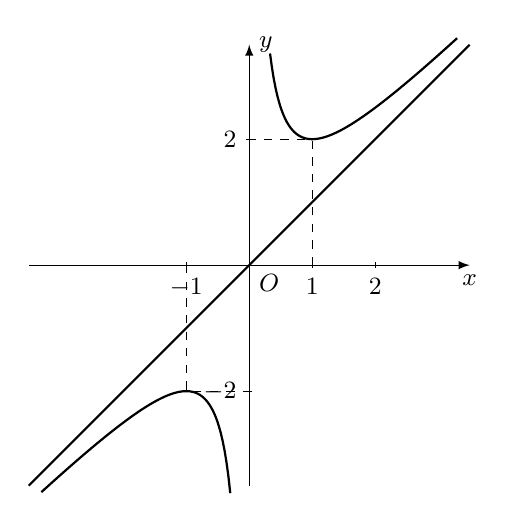
\begin{tikzpicture}[>=latex, scale=0.8]
    % 1. Hệ trục tọa độ
    \draw[->] (-3.5,0) -- (3.5,0) node[below] {\small $x$};
    \draw[->] (0,-3.5) -- (0,3.5) node[right] {\small $y$};
    \node[below right] at (0,0) {\small $O$};
    
    % 2. Đánh dấu các mốc
    \foreach \x in {-1,1,2} {
        \draw (\x,0.05) -- (\x,-0.05) node[below] {\small $\x$};
    }
    \foreach \val in {-2,2} {
        \draw (0.05,\val) -- (-0.05,\val) node[left] {\small $\val$};
    }
    
    % 3. Vẽ đồ thị hàm số
    \draw[thick, samples=100, domain=-3.3:-0.3] 
        plot (\x, {\x + 1/\x});
    \draw[thick, samples=100, domain=0.33:3.3] 
        plot (\x, {\x + 1/\x});
    \draw[thick, samples=100, domain=-3.5:3.5] 
        plot (\x, {\x });
        \draw[dashed] (1,0) -- (1,2)-- (0,2);
        \draw[dashed] (-1,0) -- (-1,-2) -- (0,-2);
\end{tikzpicture}
\end{center}

Tâm đối xứng của đồ thị hàm số đã cho là}{
    \begin{tasks}(4)
        \task \( I(1; 2) \)
        \task \( J(-1; -2) \)
        \task \( K(1; 1) \)
        \task \( O(0; 0) \)
    \end{tasks}
}

% --- CÂU 25 ---
\questionLinesManual{3}{25}{Cho hàm số có đồ thị như hình vẽ bên dưới. Phương trình đường tiệm cận đứng và tiệm cận ngang của đồ thị hàm số là

\begin{center}
\begin{tikzpicture}[>=latex, scale=0.8]
    % 1. Hệ trục tọa độ
    \draw[->] (-3.5,0) -- (4.5,0) node[below] {\small $x$};
    \draw[->] (0,-3.5) -- (0,4.5) node[right] {\small $y$};
    \node[below left] at (0,0) {\small $O$};
    
    % 2. Đánh dấu các mốc
    \foreach \x in {1,2} {
        \draw (\x,0.05) -- (\x,-0.05) node[below] {\small $\x$};
    }
    \foreach \val in {1,2} {
        \draw (0.05,\val) -- (-0.05,\val) node[left] {\small $\val$};
    }
    
    % 3. Vẽ đồ thị hàm số y = (x+2)/(x-1)
    \draw[thick, samples=100, domain=-3.5:0.7] 
        plot (\x, {(\x - 2)/(\x - 1)});
    \draw[thick, samples=100, domain=1.23:4.5] 
        plot (\x, {(\x - 2)/(\x - 1)});
    
    % 4. Đường tiệm cận
    \draw[dashed] (1,-3.5) -- (1,4.5);
    \draw[dashed] (-3.5,1) -- (4.5,1);
\end{tikzpicture}
\end{center}

}{
    \begin{tasks}(4)
        \task \( x = 2, y = 1 \)
        \task \( x = 1, y = 2 \)
        \task \( x = 1, y = 1 \)
        \task \( x = -1, y = 1 \)
    \end{tasks}
}

% --- CÂU 26 ---
\questionLinesManual{3}{26}{Cho hàm số \( y = \dfrac{ax + b}{cx + d} \) (\(a, b, c \in \mathbb{R}\)) có đồ thị là đường cong như hình vẽ bên. Toạ độ tâm đối xứng của đồ thị hàm số đã cho là:

\begin{center}
\begin{tikzpicture}[>=latex, scale=0.8]
                % 1. Hệ trục tọa độ
                \draw[->] (-4.5,0) -- (3.5,0) node[below] {\small $x$};
                \draw[->] (0,-3.5) -- (0,4.5) node[right] {\small $y$};
                \node[below left] at (0,0) {\small $O$};
                
                % 2. Đánh dấu các mốc
                \foreach \x in {-1,1} {
                    \draw (\x,0.05) -- (\x,-0.05) node[below] {\small $\x$};
                }
                \foreach \val in {1} {
                    \draw (0.05,\val) -- (-0.05,\val) node[left] {\small $\val$};
                }
                
                % 3. Vẽ đồ thị hàm số y = (x+1)/(-x+1) = -(x+1)/(x-1)
                \draw[thick, samples=100, domain=-4.5:-1.57] 
                    plot (\x, {(\x - 1)/(\x + 1)});
                \draw[thick, samples=100, domain=-0.57:3.5] 
                    plot (\x, {(\x - 1)/(\x + 1)});
                
                % 4. Đường tiệm cận
                \draw[dashed] (-1,-3.5) -- (-1,4.5) ;
                \draw[dashed] (-4.5,1) -- (3.5,1) ;
            \end{tikzpicture}
\end{center}

}{
    \begin{tasks}(4)
        \task \((-1; 1)\)
        \task \((1; 1)\)
        \task \((1; -1)\)
        \task \((0; 1)\)
    \end{tasks}
}

% --- CÂU 27 ---
\questionLinesManual{3}{27}{Cho hàm số \( y = f(x) = \dfrac{ax^2 + bx + c}{dx + e} \) có đồ thị như hình vẽ dưới đây:

\begin{center}
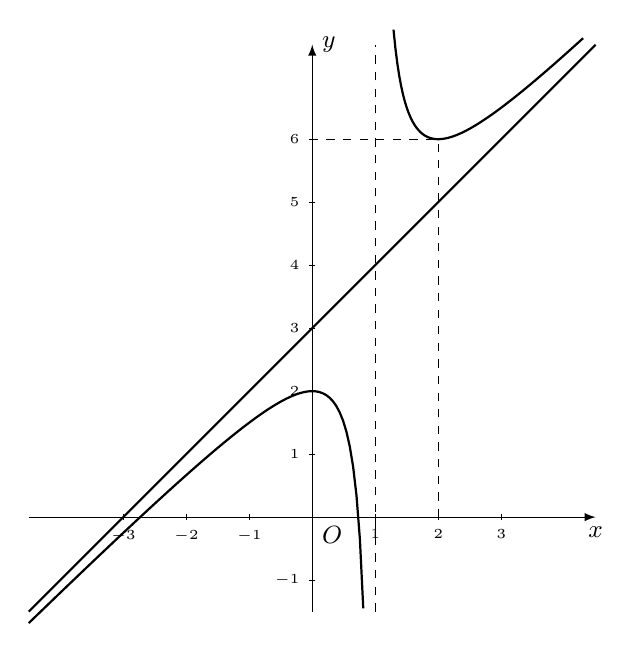
\begin{tikzpicture}[>=latex, scale=0.8]
    % 1. Hệ trục tọa độ
    \draw[->] (-4.5,0) -- (4.5,0) node[below] {\small $x$};
    \draw[->] (0,-1.5) -- (0,7.5) node[right] {\small $y$};
    \node[below right] at (0,0) {\small $O$};
    
    % 2. Đánh dấu các mốc
    \foreach \x in {-3,-2,-1,1,2,3} {
        \draw (\x,0.05) -- (\x,-0.05) node[below] {\tiny $\x$};
    }
    \foreach \val in {-1,1,2,3,4,5,6} {
        \draw (0.05,\val) -- (-0.05,\val) node[left] {\tiny $\val$};
    }
    
    % 3. Vẽ đồ thị hàm số y = (x^2 + x - 1)/(x - 1)
    \draw[thick, samples=100, domain=-4.5:0.81] 
        plot (\x, {(\x*\x - \x + 1)/(\x - 1)+3});
    \draw[thick, samples=100, domain=1.29:4.3] 
        plot (\x, {(\x*\x - \x +1)/(\x - 1)+3});
    \draw[thick, samples=100, domain=-4.5:4.5] 
        plot (\x, {(\x+3});
    % 4. Đường tiệm cận
    \draw[dashed] (1,-1.5) -- (1,7.5) ;
    \draw[dashed] (2,0) -- (2,6) -- (0,6);
\end{tikzpicture}
\end{center}

Hàm số đã cho đồng biến trên khoảng nào trong các khoảng sau?}{
    \begin{tasks}(4)
        \task \((-\infty; 1)\)
        \task \((2; +\infty)\)
        \task \((0; 1)\)
        \task \((1; 2)\)
    \end{tasks}
}

% --- CÂU 28 ---
\questionLinesManual{3}{28}{Hàm số nào sau đây có đồ thị như hình vẽ?

\begin{center}
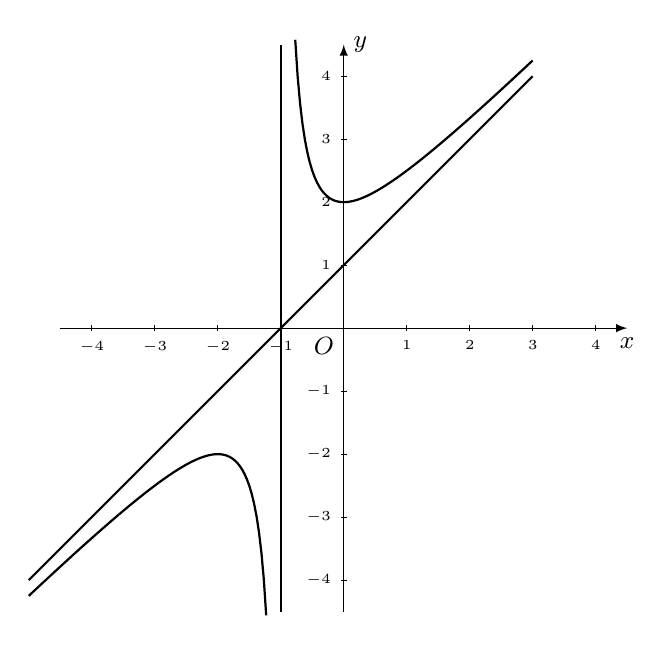
\begin{tikzpicture}[>=latex, scale=0.8]
    % 1. Hệ trục tọa độ
    \draw[->] (-4.5,0) -- (4.5,0) node[below] {\small $x$};
    \draw[->] (0,-4.5) -- (0,4.5) node[right] {\small $y$};
    \node[below left] at (0,0) {\small $O$};
    
    % 2. Đánh dấu các mốc
    \foreach \x in {-4,-3,-2,-1,1,2,3,4} {
        \draw (\x,0.05) -- (\x,-0.05) node[below] {\tiny $\x$};
    }
    \foreach \val in {-4,-3,-2,-1,1,2,3,4} {
        \draw (0.05,\val) -- (-0.05,\val) node[left] {\tiny $\val$};
    }
    
    % 3. Vẽ đồ thị hàm số y = (x^2 + 2x + 2)/(x + 1)
    \draw[thick, samples=100, domain=-5:-1.23] 
        plot (\x, {(\x*\x + 2*\x + 2)/(\x + 1)});
    \draw[thick, samples=100, domain=-0.77:3] 
        plot (\x, {(\x*\x + 2*\x + 2)/(\x + 1)});
    \draw[thick, samples=100, domain=-5:3] 
        plot (\x, {\x+1});
    
    % 4. Đường tiệm cận
    \draw[thick] (-1,-4.5) -- (-1,4.5);
\end{tikzpicture}
\end{center}

}{
    \begin{tasks}(4)
        \task \( y = \dfrac{x - 2}{x + 1} \)
        \task \( y = \dfrac{x^2 + 2x + 2}{x + 1} \)
        \task \( y = x^2 - 2x + 3 \)
        \task \( y = x^3 - 3x + 2 \)
    \end{tasks}
}

\questionLinesManual{8}{29}{Cho hàm số \( y = \dfrac{ax + b}{cx + d} \) có đồ thị như sau.

\begin{center}
\begin{tikzpicture}[>=latex, scale=0.8]
    % Vẽ hệ trục
    \draw[->] (-3.5,0) -- (5.5,0) node[below] {$x$};
    \draw[->] (0,-3.5) -- (0,5.5) node[right] {$y$};
    \node[below right] at (0,0) {$O$};
   
    % Vẽ đồ thị hàm số
    \draw[thick, samples=100, domain=-3.5:0.55] 
        plot (\x, {(\x + 1)/(\x -1)});
    \draw[thick, samples=100, domain=1.45:5.5] 
        plot (\x, {(\x + 1)/(\x - 1)});
    
    % Đường tiệm cận
    \draw[dashed] (1,-3.5) -- (1,5.5) ;
    \draw[dashed] (-3.5,1) -- (5.5,1);
\end{tikzpicture}
\end{center}

Mệnh đề nào sau đây đúng?}{
    \begin{tasks}(4)
        \task \( ac > 0; \, bd > 0 \)
        \task \( ab < 0; \, cd < 0 \)
        \task \( bc > 0; \, ad < 0 \)
        \task \( ad > 0; \, bd < 0 \)
    \end{tasks}
}

% --- CÂU 30 ---
\questionLinesManual{8}{30}{Cho hàm số \( y = \dfrac{(a-1)x + b}{(c-1)x + d} \), \( d < 0 \) có đồ thị như hình trên. Khẳng định nào dưới đây là đúng?

\begin{center}
\begin{tikzpicture}[>=latex, scale=0.8]
    % Vẽ hệ trục
    \draw[->] (-3.5,0) -- (5.5,0) node[below] {$x$};
    \draw[->] (0,-3.5) -- (0,5.5) node[right] {$y$};
    \node[below right] at (0,0) {$O$};
    
    % Vẽ đồ thị hàm số
    \draw[thick, samples=100, domain=-3.5:0.55] 
        plot (\x, {(\x + 1)/(\x -1)});
    \draw[thick, samples=100, domain=1.45:5.5] 
        plot (\x, {(\x + 1)/(\x -1)});
    
    % Đường tiệm cận
    \draw[dashed] (1,-3.5) -- (1,5.5);
    \draw[dashed] (-3.5,1) -- (5.5,1);
\end{tikzpicture}
\end{center}

}{
    \begin{tasks}(4)
        \task \( a > 1, b > 0, c < 1 \)
        \task \( a > 1, b < 0, c > 1 \)
        \task \( a < 1, b > 0, c < 1 \)
        \task \( a > 1, b > 0, c > 1 \)
    \end{tasks}
}

% --- CÂU 31 ---
\questionLinesManual{8}{31}{Cho hàm số \( y = \dfrac{ax + b}{cx + d} \) có đồ thị như trong hình bên dưới. Biết rằng \( a \) là số thực dương, hỏi trong các số \( b, c, d \) có tất cả bao nhiêu số dương?

\begin{center}
\begin{tikzpicture}[>=latex, scale=0.8]
    % Vẽ hệ trục
    \draw[->] (-5.5,0) -- (3.5,0) node[below] {$x$};
    \draw[->] (0,-2.5) -- (0,6.5) node[right] {$y$};
    \node[below left] at (0,0) {$O$};
    % Vẽ đồ thị hàm số
    \draw[thick, samples=100, domain=-5.5:-1.7] 
        plot (\x, {(2*\x - 1)/(\x + 1)});
    \draw[thick, samples=100, domain=-0.35:3.5] 
        plot (\x, {(2*\x - 1)/(\x + 1)});
    
    % Đường tiệm cận
    \draw[dashed] (-1,-2.5) -- (-1,6.5);
    \draw[dashed] (-5.5,2) -- (3.5,2);
\end{tikzpicture}
\end{center}

}{
    \begin{tasks}(4)
        \task $1$
        \task $2$
        \task $0$
        \task $3$
    \end{tasks}
}

% --- CÂU 32 ---
\questionLinesManual{8}{32}{Cho hàm số \( y = \dfrac{ax + b}{cx + d} \) có đồ thị như hình vẽ bên. Khẳng định nào sau đây là khẳng định đúng?

\begin{center}
\begin{tikzpicture}[>=latex, scale=0.5]
    % Vẽ hệ trục
    \draw[->] (-7.5,0) -- (4.5,0) node[below] {$x$};
    \draw[->] (0,-4.5) -- (0,6.5) node[right] {$y$};
    \node[below left] at (0,0) {$O$};
    
    % Vẽ đồ thị hàm số
    \draw[thick, samples=100, domain=-7.5:-2.55] 
        plot (\x, {(\x - 1)/(\x + 2)});
    \draw[thick, samples=100, domain=-1.45:4.5] 
        plot (\x, {(\x - 1)/(\x + 2)});
    
    % Đường tiệm cận
    \draw[dashed] (-2,-4.5) -- (-2,6.5);
    \draw[dashed] (-7.5,1) -- (4.5,1);
\end{tikzpicture}
\end{center}

}{
    \begin{tasks}(4)
        \task 
        \(\begin{cases} 
        ad < 0 \\ 
        bc > 0 
        \end{cases}\)
        \task 
        \(\begin{cases} 
        ad < 0 \\ 
        bc < 0 
        \end{cases}\)
        \task 
        \(\begin{cases} 
        ad > 0 \\ 
        bc < 0 
        \end{cases}\)
        \task 
        \(\begin{cases} 
        ad > 0 \\ 
        bc > 0 
        \end{cases}\)
    \end{tasks}
}

% --- CÂU 33 ---
\questionLinesManual{8}{33}{Hình vẽ bên là đồ thị hàm số \( y = \dfrac{ax + b}{cx + d} \). Mệnh đề nào dưới đây đúng?

\begin{center}
\begin{tikzpicture}[>=latex, scale=0.8]
    % Vẽ hệ trục
    \draw[->] (-5.5,0) -- (3.5,0) node[below] {$x$};
    \draw[->] (0,-3.5) -- (0,5.5) node[right] {$y$};
    \node[below left] at (0,0) {$O$};
    
    % Vẽ đồ thị hàm số
    \draw[thick, samples=100, domain=-5.5:-1.33] 
        plot (\x, {(\x - 0.5)/(\x + 1)});
    \draw[thick, samples=100, domain=-0.67:3.5] 
        plot (\x, {(\x - 0.5)/(\x + 1)});
    
    % Đường tiệm cận
    \draw[dashed] (-1,-3.5) -- (-1,5.5);
    \draw[dashed] (-5.5,1) -- (3.5,1);
\end{tikzpicture}
\end{center}

}{
    \begin{tasks}(4)
        \task \( ad > 0 \) và \( bd > 0 \)
        \task \( ad > 0 \) và \( ab < 0 \)
        \task \( bd < 0 \) và \( ab > 0 \)
        \task \( ad < 0 \) và \( ab < 0 \)
    \end{tasks}
}

% --- CÂU 34 ---
\questionLinesManual{8}{34}{Cho hàm số \( y = \dfrac{ax - b}{x - 1} \) có đồ thị như hình vẽ dưới đây:

\begin{center}
\begin{tikzpicture}[>=latex, scale=0.6]
    % Vẽ hệ trục
    \draw[->] (-3.5,0) -- (5.5,0) node[below] {\tiny$x$};
    \draw[->] (0,-5.5) -- (0,3.5) node[right] {\tiny$y$};
    \node[below left] at (0,0) {\tiny$O$};
    
    % Đánh dấu các mốc
    \foreach \x in {1,2} {
        \draw (\x,0.1) -- (\x,-0.1) node[below left] {\tiny$\x$};
    }
    \foreach \y in {-2,-1} {
        \draw (0.1,\y) -- (-0.1,\y) node[below left] {\tiny$\y$};
    }
    
    % Vẽ đồ thị hàm số
    \draw[thick, samples=100, domain=-3.5:0.78] 
        plot (\x, {(-\x +2)/(\x - 1)});
    \draw[thick, samples=100, domain=1.22:5.5] 
        plot (\x, {(-\x + 2)/(\x - 1)});
    
    % Đường tiệm cận
    \draw[dashed] (1,-5.5) -- (1,3.5);
    \draw[dashed] (-3.5,-1) -- (5.5,-1);
\end{tikzpicture}
\end{center}

Khẳng định nào sau đây đúng?}{
    \begin{tasks}(4)
        \task \( b < a < 0 \)
        \task \( a < b < 0 \)
        \task \( b > a \) và \( a < 0 \)
        \task \( a < 0 < b \)
    \end{tasks}
}



% --- CÂU 29 ---
\questionLinesManual{8}{35}{Cho hàm số \( y = \dfrac{x^2 + bx + c}{mx + n} \) (\( m \neq 0 \))  có đồ thị là đường cong bên dưới

\begin{center}
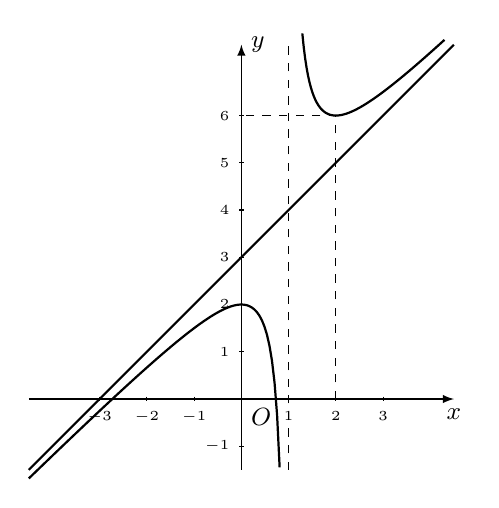
\begin{tikzpicture}[>=latex, scale=0.6]
    % 1. Hệ trục tọa độ
    \draw[->] (-4.5,0) -- (4.5,0) node[below] {\small $x$};
    \draw[->] (0,-1.5) -- (0,7.5) node[right] {\small $y$};
    \node[below right] at (0,0) {\small $O$};
    
    % 2. Đánh dấu các mốc
    \foreach \x in {-3,-2,-1,1,2,3} {
        \draw (\x,0.05) -- (\x,-0.05) node[below] {\tiny $\x$};
    }
    \foreach \val in {-1,1,2,3,4,5,6} {
        \draw (0.05,\val) -- (-0.05,\val) node[left] {\tiny $\val$};
    }
    
    % 3. Vẽ đồ thị hàm số y = (x^2 + x - 1)/(x - 1)
    \draw[thick, samples=100, domain=-4.5:0.81] 
        plot (\x, {(\x*\x - \x + 1)/(\x - 1)+3});
    \draw[thick, samples=100, domain=1.29:4.3] 
        plot (\x, {(\x*\x - \x +1)/(\x - 1)+3});
    \draw[thick, samples=100, domain=-4.5:4.5] 
        plot (\x, {(\x+3});
    % 4. Đường tiệm cận
    \draw[dashed] (1,-1.5) -- (1,7.5) ;
    \draw[dashed] (2,0) -- (2,6) -- (0,6);
\end{tikzpicture}
\end{center}

Trong các số \( b, c, m, n \) có tất cả bao nhiêu số dương?}{
    \begin{tasks}(4)
        \task $1$
        \task $2$
        \task $3$
        \task $4$
    \end{tasks}
}

% --- CÂU 30 ---
\questionLinesManual{8}{36}{Cho hàm số \( y = \dfrac{ax^2 + bx + c}{x + d} \) (\( a \neq 0 \))  có đồ thị như hình vẽ sau:

\begin{center}
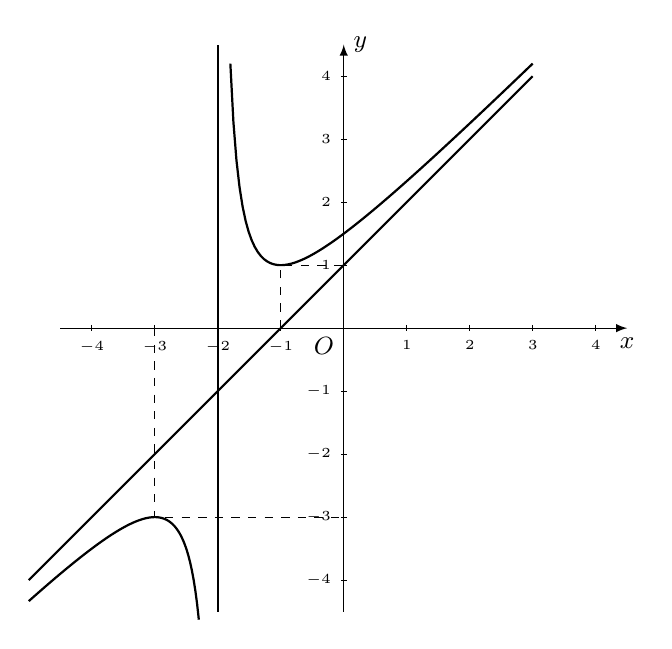
\begin{tikzpicture}[>=latex, scale=0.8]
    % 1. Hệ trục tọa độ
    \draw[->] (-4.5,0) -- (4.5,0) node[below] {\small $x$};
    \draw[->] (0,-4.5) -- (0,4.5) node[right] {\small $y$};
    \node[below left] at (0,0) {\small $O$};
    
    % 2. Đánh dấu các mốc
    \foreach \x in {-4,-3,-2,-1,1,2,3,4} {
        \draw (\x,0.05) -- (\x,-0.05) node[below] {\tiny $\x$};
    }
    \foreach \val in {-4,-3,-2,-1,1,2,3,4} {
        \draw (0.05,\val) -- (-0.05,\val) node[left] {\tiny $\val$};
    }
    
    % 3. Vẽ đồ thị hàm số y = (x^2 + 2x + 2)/(x + 1)
    \draw[thick, samples=100, domain=-5:-2.3] 
        plot (\x, {(\x*\x + 3*\x + 3)/(\x + 2)});
    \draw[thick, samples=100, domain=-1.8:3] 
        plot (\x, {(\x*\x + 3*\x + 3)/(\x + 2)});
    \draw[thick, samples=100, domain=-5:3] 
        plot (\x, {\x+1});
    
    % 4. Đường tiệm cận
    \draw[thick] (-2,-4.5) -- (-2,4.5);
    \draw [dashed] (-1,0) -- (-1,1) --(0,1);
    \draw[dashed] (-3,0) -- (-3,-3) --( 0,-3);
\end{tikzpicture}
\end{center}

Trong các số \( a, b, c, d \) có tất cả bao nhiêu số dương?}{
    \begin{tasks}(4)
        \task $1$
        \task $2$
        \task $3$
        \task $4$
    \end{tasks}
}

% --- CÂU 31 ---
\questionLinesManual{8}{37}{Cho hàm số \( y = \dfrac{ax^2 + bx + c}{a'x + b'} \) (\(a>0, a' \neq 0 \))  có đồ thị như hình vẽ bên. Hàm số đã cho nghịch biến trên khoảng nào trong các khoảng sau đây?

\begin{center}
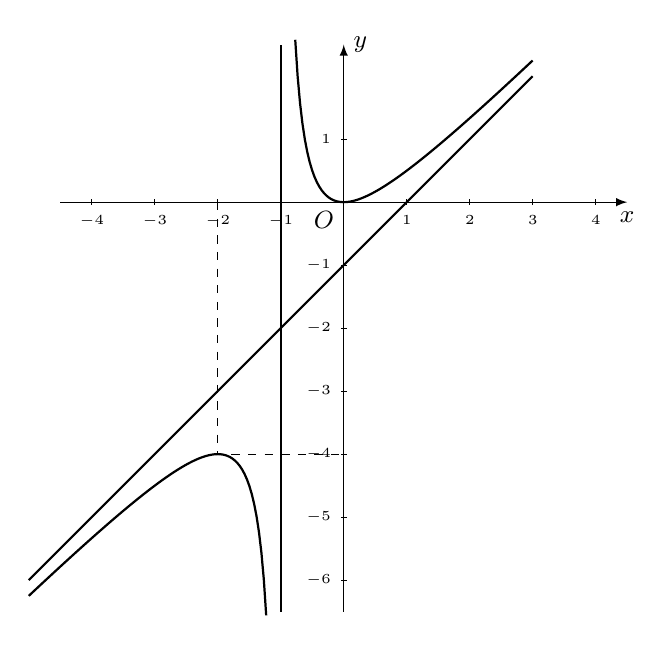
\begin{tikzpicture}[>=latex, scale=0.8]
    % 1. Hệ trục tọa độ
    \draw[->] (-4.5,0) -- (4.5,0) node[below] {\small $x$};
    \draw[->] (0,-6.5) -- (0,2.5) node[right] {\small $y$};
    \node[below left] at (0,0) {\small $O$};
    
    % 2. Đánh dấu các mốc
    \foreach \x in {-4,-3,-2,-1,1,2,3,4} {
        \draw (\x,0.05) -- (\x,-0.05) node[below] {\tiny $\x$};
    }
    \foreach \val in {,-6,-5,-4,-3,-2,-1,1,} {
        \draw (0.05,\val) -- (-0.05,\val) node[left] {\tiny $\val$};
    }
    
    % 3. Vẽ đồ thị hàm số y = (x^2 + 2x + 2)/(x + 1)
    \draw[thick, samples=100, domain=-5:-1.23] 
        plot (\x, {(\x*\x + 2*\x + 2)/(\x + 1)-2});
    \draw[thick, samples=100, domain=-0.77:3] 
        plot (\x, {(\x*\x + 2*\x + 2)/(\x + 1)-2});
    \draw[thick, samples=100, domain=-5:3] 
        plot (\x, {\x-1});
    \draw[dashed] (-2,0) -- (-2,-4) --(0,-4);
    % 4. Đường tiệm cận
    \draw[thick] (-1,-6.5) -- (-1,2.5);
\end{tikzpicture}
\end{center}

Trong các số \( b, c, a', b' \) có tất cả bao nhiêu số dương?}{
    \begin{tasks}(4)
        \task $1$
        \task $2$
        \task $3$
        \task $4$
    \end{tasks}
}

\newpage

% --- CÂU 32 ---
\questionLinesManual{8}{38}{Cho hàm số \( y = ax + b - \dfrac{r}{x} \) (\(ab  \neq 0\)) và có đồ thị là \( (C) \) có dạng như hình vẽ sau.

\begin{center}
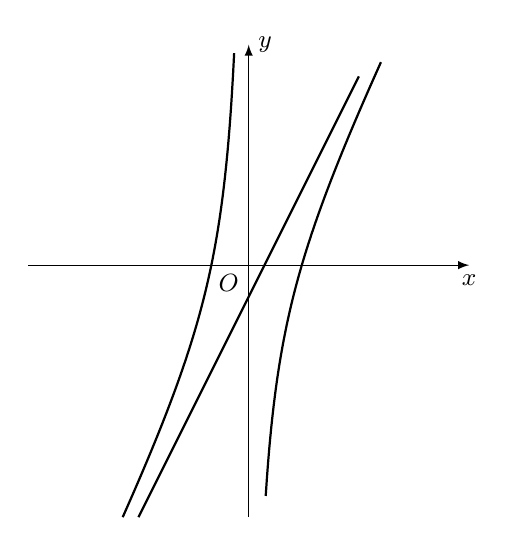
\begin{tikzpicture}[>=latex, scale=0.8]
    % 1. Hệ trục tọa độ
    \draw[->] (-3.5,0) -- (3.5,0) node[below] {\small $x$};
    \draw[->] (0,-4) -- (0,3.5) node[right] {\small $y$};
    \node[below left] at (0,0) {\small $O$};
   
    % 3. Vẽ đồ thị hàm số y = x + 1 - 2/x
    \draw[thick, samples=100, domain=-2:-0.23] 
        plot (\x, {2*\x  - 1/\x-0.5});
    \draw[thick, samples=100, domain=0.27:2.1] 
        plot (\x, {2*\x - 1/\x-0.5});
         \draw[thick, samples=100, domain=-1.75:1.75] 
        plot (\x, {2*\x-0.5 });
\end{tikzpicture}
\end{center}

Các hệ số \( a, b, r \) phải thỏa mãn điều kiện nào dưới đây.}{
    \begin{tasks}(4)
        \task 
        \(\begin{cases} 
        a > 0 \\ 
        b < 0 \\ 
        r > 0 
        \end{cases}\)
        \task 
        \(\begin{cases} 
        a > 0 \\ 
        b > 0 \\ 
        r < 0 
        \end{cases}\)
        \task 
        \(\begin{cases} 
        a < 0 \\ 
        b > 0 \\ 
        r > 0 
        \end{cases}\)
        \task 
        \(\begin{cases} 
        a > 0 \\ 
        b < 0 \\ 
        r < 0 
        \end{cases}\)
    \end{tasks}
}

% --- CÂU 33 ---
\questionLinesManual{8}{39}{Cho hàm số \( y = \dfrac{ax^2 + bx + c}{mx + n} \) (\( a > 0, m \neq 0 \)) có đồ thị như hình vẽ bên.

\begin{center}
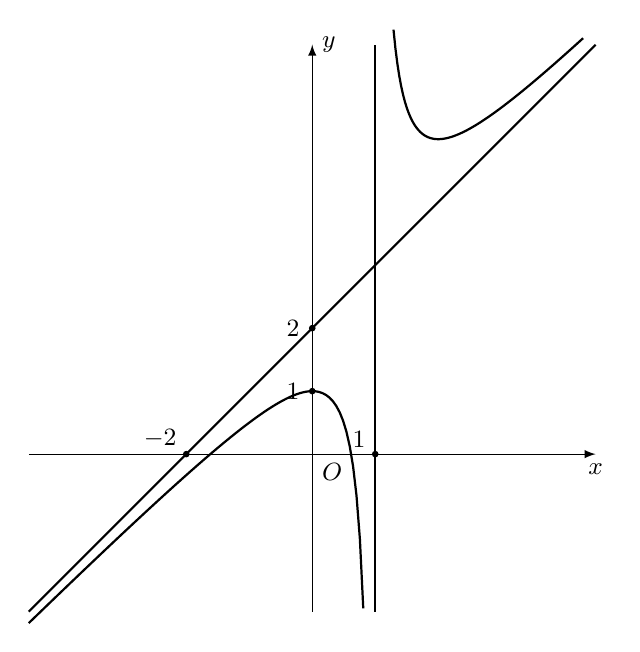
\begin{tikzpicture}[>=latex, scale=0.8]
    % 1. Hệ trục tọa độ
    \draw[->] (-4.5,0) -- (4.5,0) node[below] {\small $x$};
    \draw[->] (0,-2.5) -- (0,6.5) node[right] {\small $y$};
    \node[below right] at (0,0) {\small $O$};
    
    % 2. Đánh dấu các mốc
    \foreach \x in {-2,1} {
        \draw (\x,0.05) -- (\x,-0.05) node[above left] {\small $\x$};
    }
    \foreach \val in {1,2} {
        \draw (0.05,\val) -- (-0.05,\val) node[left] {\small $\val$};
    }
    
    % 3. Vẽ đồ thị hàm số y = (x^2 + x - 1)/(x - 1)
    \draw[thick, samples=100, domain=-4.5:0.81] 
        plot (\x, {(\x*\x - \x + 1)/(\x - 1)+2});
    \draw[thick, samples=100, domain=1.29:4.3] 
        plot (\x, {(\x*\x - \x +1)/(\x - 1)+2});
    \draw[thick, samples=100, domain=-4.5:4.5] 
        plot (\x, {(\x+2)});
    % 4. Đường tiệm cận
    \draw[thick] (1,-2.5) -- (1,6.5) ;
    \fill (0,2) circle (1.5pt);
    \fill (0,1) circle (1.5pt);
    \fill (-2,0) circle (1.5pt);
    \fill (1,0) circle (1.5pt);
\end{tikzpicture}
\end{center}

Trong các số \( b, c, m, n \) có tất cả bao nhiêu số dương?}{
    \begin{tasks}(4)
        \task $1$
        \task $2$
        \task $3$
        \task $4$
    \end{tasks}
}

% --- CÂU 34 ---
\questionLinesManual{3}{40}{Tập xác định của hàm số \( f(x) = \dfrac{x^2 - 4x - 3}{x + 3} \) là}{
    \begin{tasks}(4)
        \task \( D = \mathbb{R} \setminus \{3\} \)
        \task \( D = \mathbb{R} \setminus \{0\} \)
        \task \( D = \mathbb{R} \)
        \task \( D = \mathbb{R} \setminus \{-3\} \)
    \end{tasks}
}

% --- CÂU 35 ---
\questionLinesManual{5}{41}{Giá trị nhỏ nhất của hàm số \( y = x - 3 + \dfrac{9}{x + 2} \) trên đoạn \([-1; 3]\) bằng}{
    \begin{tasks}(4)
        \task $0$
        \task $5$
        \task $1$
        \task $\dfrac{9}{5}$
    \end{tasks}
}

% --- CÂU 36 ---
\questionLinesManual{8}{42}{Đường thẳng qua 2 điểm cực trị của đồ thị hàm số \( y = \dfrac{x^2 - x + 2}{x + 2} \) có phương trình là}{
    \begin{tasks}(4)
        \task \( y = 2x - 1 \)
        \task \( y = 2x + 1 \)
        \task \( y = x - 2 \)
        \task \( y = -2x - 1 \)
    \end{tasks}
}

% --- CÂU 37 ---
\questionLinesManual{8}{43}{Cho hàm số \( y = \dfrac{x^2 + 3x + 3}{x + 1} \) có đồ thị \((C)\). Tiếp tuyến của đồ thị \((C)\) tại giao điểm của đồ thị với trục tung cắt đường tiệm cận xiên của đồ thị tại điểm có tọa độ là}{
    \begin{tasks}(4)
        \task $(1; 2)$
        \task $(1; 3)$
        \task $(-1; 1)$
        \task $(-1; 3)$
    \end{tasks}
}

% --- CÂU 38 ---
\questionLinesManual{8}{44}{Phương trình tiếp tuyến của đồ thị hàm số \( y = \dfrac{x - 2}{x + 1} \) tại điểm có tung độ \(y_0 = -2\) là}{
    \begin{tasks}(4)
        \task \( y = 3x - 2 \)
        \task \( y = -3x + 2 \)
        \task \( y = 3x + 2 \)
        \task \( y = -3x - 2 \)
    \end{tasks}
}

% --- CÂU 39 ---
\questionLinesManual{8}{45}{Cho hàm số \( y = \dfrac{x - 1}{x + 1} \) có đồ thị \((C)\). Có bao nhiêu điểm thuộc đồ thị \((C)\) sao cho tiếp tuyến của đồ thị \((C)\) tại các điểm đó song song với đường thẳng \(y = 2x + 7\)?}{
    \begin{tasks}(4)
        \task $2$
        \task $1$
        \task $0$
        \task $3$
    \end{tasks}
}

% --- CÂU 40 ---
\questionLinesManual{8}{46}{Cho hàm số \( y = \dfrac{2x - 1}{x + 1} \) (C). Tiếp tuyến của (C) vuông góc với đường thẳng \( x + 3y + 2 = 0 \) tại điểm có hoành độ là}{
    \begin{tasks}(4)
        \task \( x = 0 \)
        \task \( x = -2 \)
        \task 
        \(\begin{cases} 
        x = 0 \\ 
        x = -2 
        \end{cases}\)
        \task 
        \(\begin{cases} 
        x = 0 \\ 
        x = 2 
        \end{cases}\)
    \end{tasks}
}

% --- CÂU 1: HÀM BẬC 3 ---
\questionLinesManual{5}{47}{Cho hàm số \( y = x^3 - 3x^2 + 2 \). Tìm tọa độ tâm đối xứng của đồ thị hàm số.}{
    \begin{tasks}(4)
        \task \( I(1; 0) \)
        \task \( I(1; 2) \)
        \task \( I(1; -2) \)
        \task \( I(0; 2) \)
    \end{tasks}
}

% --- CÂU 2: HÀM BẬC 3 ---
\questionLinesManual{5}{48}{Cho hàm số \( y = -2x^3 + 6x^2 - 4x + 1 \). Tâm đối xứng của đồ thị hàm số có tung độ bằng:}{
    \begin{tasks}(4)
        \task \( 1 \)
        \task \( -1 \)
        \task \( 3 \)
        \task \( -3 \)
    \end{tasks}
}

% --- CÂU 3: HÀM B1/B1 ---
\questionLinesManual{3}{49}{Cho hàm số \( y = \dfrac{2x + 1}{x - 1} \). Tâm đối xứng của đồ thị hàm số là:}{
    \begin{tasks}(4)
        \task \( I(1; 2) \)
        \task \( I(1; -2) \)
        \task \( I(-1; 2) \)
        \task \( I(2; 1) \)
    \end{tasks}
}

% --- CÂU 4: HÀM B1/B1 ---
\questionLinesManual{3}{50}{Cho hàm số \( y = \dfrac{-x + 3}{x + 2} \). Tổng hoành độ và tung độ của tâm đối xứng là:}{
    \begin{tasks}(4)
        \task \( 1 \)
        \task \( -1 \)
        \task \( 3 \)
        \task \( -3 \)
    \end{tasks}
}

% --- CÂU 5: HÀM B2/B1 ---
\questionLinesManual{5}{51}{Cho hàm số \( y = \dfrac{x^2 + 2x + 2}{x + 1} \). Tâm đối xứng của đồ thị hàm số là:}{
    \begin{tasks}(4)
        \task \( I(-1; 0) \)
        \task \( I(-1; 1) \)
        \task \( I(-1; 2) \)
        \task \( I(1; 1) \)
    \end{tasks}
}

% --- CÂU 6: HÀM B2/B1 ---
\questionLinesManual{5}{52}{Cho hàm số \( y = \dfrac{x^2 - 4x + 5}{x - 2} \). Tọa độ tâm đối xứng của đồ thị hàm số là:}{
    \begin{tasks}(4)
        \task \( I(2; 0) \)
        \task \( I(2; 2) \)
        \task \( I(2; -2) \)
        \task \( I(0; 2) \)
    \end{tasks}
}

% --- CÂU 42 ---
\questionTrueFalse{8}{53}{Cho hàm số \( y = f(x) = \dfrac{ax - 1}{bx + c} \) với \( a, b, c \in \mathbb{R} \) có bảng biến thiên như hình vẽ dưới đây

\begin{flushleft}
\begin{tikzpicture}
    \tkzTabInit[lgt=0.8, espcl=2]
    {$x$ /0.6, $f'(x)$ /0.6, $f(x)$ /1.5}
    {$-\infty$, $3$, $+\infty$}
    \tkzTabLine{, -, d, -, }
    \tkzTabVar{+/ $\dfrac{1}{2}$ / , -D+/ $-\infty$ / $+\infty$ , -/ $\dfrac{1}{2}$ /}
\end{tikzpicture}
\end{flushleft}

}{
    \textbf{a)} & Đồ thị cắt trục tung tại điểm có tung độ nhỏ hơn \( \dfrac{1}{2} \).
    & \textcolor{amberorange}{$\bigcirc$} & \textcolor{amberorange}{$\bigcirc$} \\ \hline
    
    \textbf{b)} & Đồ thị hàm số có tiệm cận đứng \( x = \dfrac{1}{2} \).
    & \textcolor{amberorange}{$\bigcirc$} & \textcolor{amberorange}{$\bigcirc$} \\ \hline
    
    \textbf{c)} & Hàm số nghịch biến trên khoảng \( (-\infty; 3) \).
    & \textcolor{amberorange}{$\bigcirc$} & \textcolor{amberorange}{$\bigcirc$} \\ \hline
    
    \textbf{d)} & \( c \in (-\infty; -2) \cup (0; +\infty) \).
    & \textcolor{amberorange}{$\bigcirc$} & \textcolor{amberorange}{$\bigcirc$} \\
}

% % --- CÂU 43 ---
% \questionTrueFalse{8}{43}{Cho hàm số \( y = f(x) = \dfrac{ax^2 + bx + 1}{cx + d} \) đạt cực đại tại \( x = 0 \) và có đồ thị như hình vẽ sau:

% \begin{flushleft}
% \begin{tikzpicture}[>=latex, scale=0.4]
%     % 1. Hệ trục tọa độ
%     \draw[->] (-4.5,0) -- (4.5,0) node[below] {\tiny $x$};
%     \draw[->] (0,-4.5) -- (0,4.5) node[right] {\tiny $y$};
%     \node[below right] at (0,0) {\tiny $O$};
    
%     % 2. Đánh dấu các mốc
%     \foreach \x in {-4,-3,-2,-1,1,2,3,4} {
%         \draw (\x,0.05) -- (\x,-0.05) node[below] {\tiny $\x$};
%     }
%     \foreach \val in {-4,-3,-2,-1,1,2,3,4} {
%         \draw (0.05,\val) -- (-0.05,\val) node[left] {\tiny $\val$};
%     }
    
%     % 3. Vẽ đồ thị hàm số y = (x^2 + x - 1)/(x - 1)
%     \draw[thick, samples=100, domain=-4.5:0.81] 
%         plot (\x, {(\x*\x - \x + 1)/(\x - 1)});
%     \draw[thick, samples=100, domain=1.29:4.3] 
%         plot (\x, {(\x*\x - \x +1)/(\x - 1)});
%     \draw[thick, samples=100, domain=-4.5:4.5] 
%         plot (\x, {(\x});
%     % 4. Đường tiệm cận
%     \draw[thick] (1,-4.5) -- (1,4.5) ;
    
% \end{tikzpicture}
% \end{flushleft}

% }{
%     \textbf{a)} & Giá trị của biểu thức \( a + b + c + d = 0 \).
%     & \textcolor{amberorange}{$\bigcirc$} & \textcolor{amberorange}{$\bigcirc$} \\ \hline
    
%     \textbf{b)} & Hàm số đồng biến trên \((-1; 0)\).
%     & \textcolor{amberorange}{$\bigcirc$} & \textcolor{amberorange}{$\bigcirc$} \\ \hline
    
%     \textbf{c)} & Gọi \( A, B \) là các điểm cực trị của đồ thị hàm số; \( M \) là điểm di động trên trục \( Ox \) sao cho góc \( AMB \) không tù. Giá trị nhỏ nhất của hoành độ điểm \( M \) là 3.
%     & \textcolor{amberorange}{$\bigcirc$} & \textcolor{amberorange}{$\bigcirc$} \\ \hline
    
%     \textbf{d)} & Đường thẳng đi qua hai điểm cực trị của hàm số có phương trình: \( y = x - 1 \).
%     & \textcolor{amberorange}{$\bigcirc$} & \textcolor{amberorange}{$\bigcirc$} \\
% }

% --- CÂU 44 ---
\questionTrueFalse{8}{54}{Cho hàm số \( y = f(x) = \dfrac{ax^2 + bx + c}{mx + n} \) (với \( a, m \neq 0 \)) có đồ thị là đường cong như Hình.

\begin{flushleft}
\begin{tikzpicture}[>=latex, scale=0.4]
    % 1. Hệ trục tọa độ
    \draw[->] (-4.5,0) -- (4.5,0) node[below] {\tiny $x$};
    \draw[->] (0,-4.5) -- (0,4.5) node[right] {\tiny $y$};
    \node[below left] at (0,0) {\tiny $O$};
    
    % 2. Đánh dấu các mốc
    \foreach \x in {-4,-3,-2,-1,1,2,3,4} {
        \draw (\x,0.05) -- (\x,-0.05) node[below] {\tiny $\x$};
    }
    \foreach \val in {-4,-3,-2,-1,1,2,3,4} {
        \draw (0.05,\val) -- (-0.05,\val) node[left] {\tiny $\val$};
    }
    
    % 3. Vẽ đồ thị hàm số y = (x^2 + 2x + 2)/(x + 1)
    \draw[thick, samples=100, domain=-5:-2.3] 
        plot (\x, {(\x*\x + 3*\x + 3)/(\x + 2)});
    \draw[thick, samples=100, domain=-1.8:3] 
        plot (\x, {(\x*\x + 3*\x + 3)/(\x + 2)});
    \draw[thick, samples=100, domain=-5:3] 
        plot (\x, {\x+1});
    
    % 4. Đường tiệm cận
    \draw[thick] (-2,-4.5) -- (-2,4.5);
    \draw [dashed] (-1,0) -- (-1,1) --(0,1);
    \draw[dashed] (-3,0) -- (-3,-3) --( 0,-3);
\end{tikzpicture}
\end{flushleft}

}{
    \textbf{a)} & Hàm số đồng biến trên các khoảng \((-\infty; -3)\) và \((-1; +\infty)\).
    & \textcolor{amberorange}{$\bigcirc$} & \textcolor{amberorange}{$\bigcirc$} \\ \hline
    
    \textbf{b)} & \( f(2024) < f(2025) \).
    & \textcolor{amberorange}{$\bigcirc$} & \textcolor{amberorange}{$\bigcirc$} \\ \hline
    \textbf{c)} & Đồ thị hàm số có tiệm cận đứng: \( x = -3 \) và đường tiệm cận xiên: \( y = x + 1 \).
    & \textcolor{amberorange}{$\bigcirc$} & \textcolor{amberorange}{$\bigcirc$} \\ \hline
    
    \textbf{d)} & Đồ thị hàm số đi qua điểm \( A\left(2; \dfrac{13}{4}\right) \).
    & \textcolor{amberorange}{$\bigcirc$} & \textcolor{amberorange}{$\bigcirc$} \\
}

% % --- CÂU 45 ---
% \questionTrueFalse{8}{45}{Cho hàm số \( f(x) = 
% \begin{cases} 
% \dfrac{3x-2}{2x-1} + 1 & \text{khi } x > 1 \\ 
% 12 & \text{khi } x = 1 \\ 
% \dfrac{x^2 - 3x - 1}{x - 1} & \text{khi } x < 1 
% \end{cases} \)

% }{
%     \textbf{a)} & Ba đường tiệm cận của đồ thị hàm số cắt nhau tạo thành tam giác có diện tích bằng 50.
%     & \textcolor{amberorange}{$\bigcirc$} & \textcolor{amberorange}{$\bigcirc$} \\ \hline
    
%     \textbf{b)} & Tiệm cận ngang của đồ thị hàm số là đường thẳng \( y = 12 \).
%     & \textcolor{amberorange}{$\bigcirc$} & \textcolor{amberorange}{$\bigcirc$} \\ \hline
    
%     \textbf{c)} & Hàm số liên tục tại điểm \( x = 1 \).
%     & \textcolor{amberorange}{$\bigcirc$} & \textcolor{amberorange}{$\bigcirc$} \\ \hline
    
%     \textbf{d)} & Đồ thị hàm số có tiệm cận đứng là đường thẳng \( x = 1 \).
%     & \textcolor{amberorange}{$\bigcirc$} & \textcolor{amberorange}{$\bigcirc$} \\
% }

% --- CÂU 46 ---
\questionTrueFalse{8}{55}{Cho hàm số \( f(x) = \dfrac{ax + b}{cx + d} \) với \( a, b, c, d \in \mathbb{R} \) và \( c \neq 0 \) có đồ thị hàm số \( y = f'(x) \) nhận đường thẳng \( x = -1 \) làm tiệm cận đứng như hình vẽ dưới. Biết rằng giá trị lớn nhất của hàm số \( y = f(x) \) trên đoạn \([-3; -2]\) bằng 8.

\begin{flushleft}
\begin{tikzpicture}[>=latex, scale=0.4]
    % 1. Hệ trục tọa độ
    \draw[->] (-5.5,0) -- (4.5,0) node[below] {\tiny $x$};
    \draw[->] (0,-1) -- (0,6) node[right] {\tiny $y$};
    \node[below left] at (0,0) {\tiny $O$};
    
    % 2. Đánh dấu các mốc
    \foreach \x in {-4,-3,-2,-1,1,2,3,4} {
        \draw (\x,0.05) -- (\x,-0.05) node[below] {\tiny $\x$};
    }
    \foreach \val in {1,2,3,4,5} {
        \draw (0.05,\val) -- (-0.05,\val) node[left] {\tiny $\val$};
    }
    
    % 3. Vẽ đồ thị f'(x)
    \draw[thick, samples=100, domain=-5.5:-1.7] 
        plot (\x, {3/(\x + 1)^2});
    \draw[thick, samples=100, domain=-0.3:4.5] 
        plot (\x, {3/(\x + 1)^2});
    
    % 4. Đường tiệm cận
    \draw[dashed] (-1,-1) -- (-1,6);
    
\end{tikzpicture}
\end{flushleft}

}{
    \textbf{a)} & Giá trị nhỏ nhất của hàm số \( y = f(x) \) trên đoạn \([2; 4]\) bằng 4.
    & \textcolor{amberorange}{$\bigcirc$} & \textcolor{amberorange}{$\bigcirc$} \\ \hline
    
    \textbf{b)} & \( f(-3) = 8 \).
    & \textcolor{amberorange}{$\bigcirc$} & \textcolor{amberorange}{$\bigcirc$} \\ \hline
    
    \textbf{c)} & Hàm số \( y = f(x) \) nghịch biến trên khoảng \((-1; +\infty)\).
    & \textcolor{amberorange}{$\bigcirc$} & \textcolor{amberorange}{$\bigcirc$} \\ \hline
    
    \textbf{d)} & Đồ thị hàm số \( y = f'(x) \) nhận đường thẳng \( y = 0 \) làm tiệm cận ngang.
    & \textcolor{amberorange}{$\bigcirc$} & \textcolor{amberorange}{$\bigcirc$} \\
}



% --- CÂU 48 ---
\questionTrueFalse{8}{56}{Cho hàm số \( y = f(x) = \dfrac{ax^2 + bx + c}{x + d} \) có đồ thị là đường cong như hình vẽ dưới đây, biết đường tiệm xiên của đồ thị hàm số đi qua hai điểm \( (0;1) \) và \( (1;0) \).

\begin{flushleft}
\begin{tikzpicture}[>=latex, scale=0.2]
    % 1. Hệ trục tọa độ
    \draw[->] (-10,0) -- (10,0) node[below] {\tiny $x$};
    \draw[->] (0,-7) -- (0,15) node[right] {\tiny $y$};
    \node[above left] at (0,0) {\tiny $O$};
    
    % 2. Đánh dấu các mốc
    \foreach \x in {-8,-4,-2,4,8} {
        \draw (\x,0.1) -- (\x,-0.1) node[above] {\tiny $\x$};
    }
    \foreach \val in {-4,-1,4,7,12} {
        \draw (0.1,\val) -- (-0.1,\val) node[left] {\tiny $\val$};
    }
    
    % 3. Vẽ đồ thị hàm số
    \draw[thick, samples=100, domain=-10:-2.35] 
        plot (\x, {(-\x*\x - \x - 2)/(\x + 2)});
    \draw[thick, samples=100, domain=-1.6:7] 
        plot (\x, {(-\x*\x - \x - 2)/(\x + 2)});
    \draw[thick, samples=100, domain=-10:7] 
        plot (\x, {-\x + 1});
    % 4. Đường tiệm cận
    \draw[thick] (-2,-7) -- (-2,15);
    \draw[dashed] (-4,0) -- (-4,7) -- (0,7);
\end{tikzpicture}
\end{flushleft}

}{
    \textbf{a)} & Tập xác định của hàm số là \( \mathbb{R} \setminus \{2\} \).
    & \textcolor{amberorange}{$\bigcirc$} & \textcolor{amberorange}{$\bigcirc$} \\ \hline
    
    \textbf{b)} & Hàm số đồng biến trên khoảng \( (-4;0) \).
    & \textcolor{amberorange}{$\bigcirc$} & \textcolor{amberorange}{$\bigcirc$} \\ \hline
    
    \textbf{c)} & Ta có \( a + b + c + d = -2 \).
    & \textcolor{amberorange}{$\bigcirc$} & \textcolor{amberorange}{$\bigcirc$} \\ \hline
    
    \textbf{d)} & Khoảng cách từ \( M(1; -8) \) đến đường thẳng đi qua các điểm cực trị của đồ thị hàm số bằng \( \sqrt{5} \).
    & \textcolor{amberorange}{$\bigcirc$} & \textcolor{amberorange}{$\bigcirc$} \\
}

% --- CÂU 49 ---
\questionTrueFalse{8}{57}{Cho hàm số \( y = \dfrac{x+1}{x-1} \) có đồ thị là đường cong \( (C) \). Giả sử \( A, B \) là hai điểm thuộc hai nhánh và \( AB \) đi qua tâm đối xứng của \( (C) \).}{
    \textbf{a)} & Tâm đối xứng của \( (C) \) là điểm \( I(1; -1) \).
    & \textcolor{amberorange}{$\bigcirc$} & \textcolor{amberorange}{$\bigcirc$} \\ \hline
    
    \textbf{b)} & Hàm số nghịch biến trên khoảng \( (-\infty; 1) \).
    & \textcolor{amberorange}{$\bigcirc$} & \textcolor{amberorange}{$\bigcirc$} \\ \hline
    
    \textbf{c)} & Có 1 tiếp tuyến của đồ thị \( (C) \) song song với đường thẳng \( d: y = -2x - 1 \).
    & \textcolor{amberorange}{$\bigcirc$} & \textcolor{amberorange}{$\bigcirc$} \\ \hline
    
    \textbf{d)} & Giá trị nhỏ nhất của đoạn thẳng \( AB \) bằng \( 3\sqrt{2} \).
    & \textcolor{amberorange}{$\bigcirc$} & \textcolor{amberorange}{$\bigcirc$} \\
}

% --- CÂU 50 ---
\questionTrueFalse{8}{58}{Cho hàm số \( y = f(x) = ax + b + \dfrac{c}{x+d} \) có đồ thị như hình vẽ sau:

\begin{flushleft}
\begin{tikzpicture}[>=latex, scale=0.2]
    % 1. Hệ trục tọa độ
    \draw[->] (-6,0) -- (4.5,0) node[below] {\tiny $x$};
    \draw[->] (0,-8) -- (0,8) node[right] {\tiny $y$};
    % 3. Vẽ đồ thị hàm số y = -2x - 4 - 2/(x+2)
    \draw[thick, samples=100, domain=-5.8:-2.27] 
        plot (\x, {-2*\x - 4 - 2/(\x + 2)});
    \draw[thick, samples=100, domain=-1.73:1.8] 
        plot (\x, {-2*\x - 4 - 2/(\x + 2)});
    \draw[thick, samples=100, domain=-6:2] 
        plot (\x, {-2*\x - 4 });
    % 4. Đường tiệm cận
    \draw[thick] (-2,-8) -- (-2,8);
    \node[above right] at (0,-4) {\tiny $-4$};
    \node[below left] at (0,-5) {\tiny $-5$};
    \node[below left] at (-2,0) {\tiny $-2$};
    \fill (0,-4) circle (2.5pt);
    \fill (0,-5) circle (2.5pt);
    \fill (-2,0) circle (2.5pt);
   \end{tikzpicture}
\end{flushleft}

}{
    \textbf{a)} & Đồ thị hàm số đã cho có tiệm cận đứng là đường thẳng \( x = -2 \).
    & \textcolor{amberorange}{$\bigcirc$} & \textcolor{amberorange}{$\bigcirc$} \\ \hline
    
    \textbf{b)} & Giá trị \( f(0) = -5 \).
    & \textcolor{amberorange}{$\bigcirc$} & \textcolor{amberorange}{$\bigcirc$} \\ \hline
    
    \textbf{c)} & Đồ thị hàm số đã cho có tiệm cận xiên là đường thẳng \( y = 2x - 4 \).
    & \textcolor{amberorange}{$\bigcirc$} & \textcolor{amberorange}{$\bigcirc$} \\ \hline
    
    \textbf{d)} & Hàm số đã cho là \( y = -2x - 4 - \dfrac{2}{x+2} \).
    & \textcolor{amberorange}{$\bigcirc$} & \textcolor{amberorange}{$\bigcirc$} \\
}

% % --- CÂU 51 ---Hỏi lại
% \questionTrueFalse{8}{51}{Cho hàm số \( y = \dfrac{x^2 + bx + c}{x + n} \) có đồ thị và hai đường tiệm cận \( d_1, d_2 \) như hình vẽ dưới đây.

% \begin{flushleft}
% \begin{tikzpicture}[>=latex, scale=0.4]
%     % 1. Hệ trục tọa độ
%     \draw[->] (-4.5,0) -- (4.5,0) node[below] {\tiny $x$};
%     \draw[->] (0,-5.5) -- (0,3.5) node[right] {\tiny $y$};
%     \node[below right] at (0,0) {\tiny $O$};
    
%     % 2. Đánh dấu các mốc
%     \foreach \x in {-4,-2,-1,1,3} {
%         \draw (\x,0.05) -- (\x,-0.05) node[below] {\tiny $\x$};
%     }
%     \foreach \val in {-5,-3,-1,1,2} {
%         \draw (0.05,\val) -- (-0.05,\val) node[left] {\tiny $\val$};
%     }
    
%     % 3. Vẽ đồ thị hàm số y = (x^2 + 2x + 2)/(x + 1)
%     \draw[thick, samples=100, domain=-5:-1.23] 
%         plot (\x, {(\x*\x + 2*\x + 2)/(\x + 1)-1});
%     \draw[thick, samples=100, domain=-0.77:3] 
%         plot (\x, {(\x*\x + 2*\x + 2)/(\x + 1)-1});
%     \draw[thick, samples=100, domain=-5:3] 
%         plot (\x, {\x});
%     \draw[dashed] (-2,0) -- (-2,-3) --(0,-3);
%     % 4. Đường tiệm cận
%     \draw[thick] (-1,-5.5) -- (-1,3.5);
% \end{tikzpicture}
% \end{flushleft}

% }{
%     \textbf{a)} & Đồ thị hàm số có tiệm cận đứng là \( x = -1 \).
%     & \textcolor{amberorange}{$\bigcirc$} & \textcolor{amberorange}{$\bigcirc$} \\ \hline
    
%     \textbf{b)} & Hàm số đồng biến trên khoảng \( (0; +\infty) \).
%     & \textcolor{amberorange}{$\bigcirc$} & \textcolor{amberorange}{$\bigcirc$} \\ \hline
    
%     \textbf{c)} & Điểm \( M(50; 98) \) và hai điểm cực trị của đồ thị hàm số thẳng hàng.
%     & \textcolor{amberorange}{$\bigcirc$} & \textcolor{amberorange}{$\bigcirc$} \\ \hline
    
%     \textbf{d)} & Đồ thị hàm số có một trục đối xứng là đường thẳng \( y = (p + \sqrt{q})(x + 1) - r \) (trong đó \( p, q, r \) là các số nguyên). Khi đó \( p + 10q + 15r = 90 \).
%     & \textcolor{amberorange}{$\bigcirc$} & \textcolor{amberorange}{$\bigcirc$} \\
% }

% % --- CÂU 52 ---Hỏi lại
% \questionTrueFalse{8}{52}{Cho hàm số \( y = \dfrac{ax^2 + bx + c}{mx + n} \) có đồ thị như hình vẽ sau

% \begin{flushleft}
% \begin{tikzpicture}[>=latex, scale=0.4]
%     % 1. Hệ trục tọa độ
%     \draw[->] (-4.5,0) -- (4.5,0) node[below] {\tiny $x$};
%     \draw[->] (0,-4.5) -- (0,4.5) node[right] {\tiny $y$};
%     \node[below right] at (0,0) {\tiny $O$};
    
%     % 2. Đánh dấu các mốc
%     \foreach \x in {-4,-2,-1,1,3} {
%         \draw (\x,0.05) -- (\x,-0.05) node[below] {\tiny $\x$};
%     }
%     \foreach \val in {-4,-2,-1,3,2} {
%         \draw (0.05,\val) -- (-0.05,\val) node[left] {\tiny $\val$};
%     }
    
%     % 3. Vẽ đồ thị hàm số y = (x^2 + 2x + 2)/(x + 1)
%     \draw[thick, samples=100, domain=-5:-1.23] 
%         plot (\x, {(\x*\x + 2*\x + 2)/(\x + 1)});
%     \draw[thick, samples=100, domain=-0.77:3] 
%         plot (\x, {(\x*\x + 2*\x + 2)/(\x + 1)});
%     \draw[thick, samples=100, domain=-5:3] 
%         plot (\x, {\x+1});
%     \draw[dashed] (-2,0) -- (-2,-2) --(0,-2);
%     % 4. Đường tiệm cận
%     \draw[thick] (-1,-4.5) -- (-1,4.5);
% \end{tikzpicture}
% \end{flushleft}

% }{
%     \textbf{a)} & Hàm số đã cho nghịch biến trên khoảng \((-2; 0)\).
%     & \textcolor{amberorange}{$\bigcirc$} & \textcolor{amberorange}{$\bigcirc$} \\ \hline
    
%     \textbf{b)} & Đồ thị của hàm số đã cho có tiệm cận xiên \( y = x + 1 \).
%     & \textcolor{amberorange}{$\bigcirc$} & \textcolor{amberorange}{$\bigcirc$} \\ \hline
    
%     \textbf{c)} & Gọi \( A, B \) là hai điểm cực trị của đồ thị hàm số đã cho, diện tích của tam giác \( OAB \) bằng \( 8 \) (với \( O \) là gốc tọa độ).
%     & \textcolor{amberorange}{$\bigcirc$} & \textcolor{amberorange}{$\bigcirc$} \\ \hline
    
%     \textbf{d)} & Một trục đối xứng của đồ thị đã cho là \( d: y = (x + 1)\tan\dfrac{3\pi}{8} \).
%     & \textcolor{amberorange}{$\bigcirc$} & \textcolor{amberorange}{$\bigcirc$} \\
% }

% --- CÂU 53 ---
\questionTrueFalse{8}{59}{Cho hàm số \( y = \dfrac{x^2 + 3x - 8}{x - 2} \) và đường tròn \( (C): (x + 3)^2 + (y - 1)^2 = 4 \). Gọi I là tâm đường tròn (C).}{
    \textbf{a)} & Hàm số (1) đồng biến trên khoảng \((-\infty; 0)\).
    & \textcolor{amberorange}{$\bigcirc$} & \textcolor{amberorange}{$\bigcirc$} \\ \hline
    
    \textbf{b)} & Giá trị nhỏ nhất của hàm số (1) trên đoạn \([3; 5]\) bằng \(7 + 2\sqrt{2}\).
    & \textcolor{amberorange}{$\bigcirc$} & \textcolor{amberorange}{$\bigcirc$} \\ \hline
    
    \textbf{c)} & Tổng khoảng cách từ điểm I đến hai tiệm cận của đồ thị hàm số (1) bằng \(\dfrac{10 + 3\sqrt{2}}{2}\).
    & \textcolor{amberorange}{$\bigcirc$} & \textcolor{amberorange}{$\bigcirc$} \\ \hline
    
    \textbf{d)} & Đường thẳng đi qua hai điểm cực trị của đồ thị hàm số (1) cắt đường tròn (C) tại hai điểm phân biệt \(M, N\). Diện tích tứ giác \(IMON\) bằng \(\dfrac{14}{5}\) (với O là gốc tọa độ).
    & \textcolor{amberorange}{$\bigcirc$} & \textcolor{amberorange}{$\bigcirc$} \\
}

% --- CÂU 54 ---
\questionTrueFalse{8}{60}{Cho hàm số \( y = \dfrac{mx^2 + nx + 1}{px + 2} \) có đồ thị như hình vẽ bên dưới.

\begin{flushleft}
\begin{tikzpicture}[>=latex, scale=0.4]
    % 1. Hệ trục tọa độ
    \draw[->] (-5,0) -- (3.5,0) node[below] {\tiny $x$};
    \draw[->] (0,-3.5) -- (0,5) node[right] {\tiny $y$};
    \node[below right] at (0,0) {\tiny $O$};
    
    
    % 3. Vẽ đồ thị hàm số
    \draw[thick, samples=100, domain=-4.5:-2.16] 
        plot (\x, {\x+1 - 1/(\x + 2)});
    \draw[thick, samples=100, domain=-1.65:3.5] 
        plot (\x, {\x+1 - 1/(\x + 2)});
    \draw[thick, samples=100, domain=-4.5:3.5] 
        plot (\x, {\x+1 });
    % 4. Đường tiệm cận
    \draw[dashed] (-2,-3.5) -- (-2,5);
    \node [below] at (-2,0) {\tiny $-2$};
    \node [below] at (-1,0) {\tiny $-1$};
    \node [left] at (0,1) {\tiny $1$};
    \fill (-2,0) circle (2.5pt);
    \fill (-1,0) circle (2.5pt);
    \fill (0,1) circle (2.5pt);
\end{tikzpicture}
\end{flushleft}

}{
    \textbf{a)} & Đường tiệm cận đứng của đồ thị là đường thẳng \( x = -2 \).
    & \textcolor{amberorange}{$\bigcirc$} & \textcolor{amberorange}{$\bigcirc$} \\ \hline
    
    \textbf{b)} & Hàm số nghịch biến trên khoảng \((-2; +\infty)\).
    & \textcolor{amberorange}{$\bigcirc$} & \textcolor{amberorange}{$\bigcirc$} \\ \hline
    
    \textbf{c)} & Đồ thị hàm số đi qua điểm \( A(0; 1) \).
    & \textcolor{amberorange}{$\bigcirc$} & \textcolor{amberorange}{$\bigcirc$} \\ \hline
    
    \textbf{d)} & Ta có \( 2m + 3n - p = 10 \).
    & \textcolor{amberorange}{$\bigcirc$} & \textcolor{amberorange}{$\bigcirc$} \\
}

% % --- CÂU 55 ---
% \questionTrueFalse{8}{55}{Cho hàm số \( y = \dfrac{2x+1}{x-1} \) (C). Các mệnh đề sau đây đúng hay sai}{
%     \textbf{a)} & Hàm số \( y = \dfrac{2x+1}{x-1} \) nghịch biến trên \( \mathbb{R} \setminus \{1\} \).
%     & \textcolor{amberorange}{$\bigcirc$} & \textcolor{amberorange}{$\bigcirc$} \\ \hline
    
%     \textbf{b)} & Hàm số đã cho có hai điểm cực trị.
%     & \textcolor{amberorange}{$\bigcirc$} & \textcolor{amberorange}{$\bigcirc$} \\ \hline
    
%     \textbf{c)} & Tiếp tuyến với đồ thị (C) tại điểm có hoành độ bằng 2 tạo với hai trục tọa độ một tam giác có diện tích bằng \( \dfrac{a}{b} \) (với \( a, b \in \mathbb{N} \) và \((a, b) = 1\)). Khi đó \( a - 20b = 1 \).
%     & \textcolor{amberorange}{$\bigcirc$} & \textcolor{amberorange}{$\bigcirc$} \\ \hline
    
%     \textbf{d)} & Lấy hai điểm \( A, B \) thuộc một nhánh của đồ thị (C) sao cho \( x_A > 1; x_B > 1 \) và hai điểm \( C, D \) thuộc đường thẳng \( \Delta: y = -x + 1 \). Khi \( ABCD \) là hình vuông thì diện tích hình vuông đó (làm tròn đến hàng phần chục) là \( 23,7 \) đơn vị diện tích.
%     & \textcolor{amberorange}{$\bigcirc$} & \textcolor{amberorange}{$\bigcirc$} \\
% }

% --- CÂU 56 ---
\questionTrueFalse{8}{61}{Cho hàm số \( y = f(x) = \dfrac{ax + b}{cx + 1} \) với \( a, b, c \in \mathbb{R} \) có đồ thị như hình vẽ dưới:

\begin{flushleft}
\begin{tikzpicture}[>=latex, scale=0.4]
    % 1. Hệ trục tọa độ
    \draw[->] (-4.5,0) -- (4.5,0) node[below] {\tiny $x$};
    \draw[->] (0,-4.5) -- (0,2.5) node[right] {\tiny $y$};
    \node[below left] at (0,0) {\tiny $O$};
   % 2. Đánh dấu các mốc
    \foreach \x in {1,2} {
        \draw (\x,0.05) -- (\x,-0.05) node[below] {\tiny $\x$};
    }
    \foreach \val in {-2,-1} {
        \draw (0.05,\val) -- (-0.05,\val) node[left] {\tiny $\val$};
    }
    % 3. Vẽ đồ thị hàm số y = (2x-1)/(x-1)
    \draw[thick, samples=100, domain=-4.5:0.7] 
        plot (\x, {(-\x +2)/(\x - 1)});
    \draw[thick, samples=100, domain=1.3:4.5] 
         plot (\x, {(-\x +2)/(\x - 1)});
    
    % 4. Đường tiệm cận
    \draw[dashed] (1,-4.5) -- (1,2.5) ;
    \draw[dashed] (-4.5,-1) -- (4.5,-1) ;
\end{tikzpicture}
\end{flushleft}

}{
    \textbf{a)} & Đạo hàm của hàm số \( f'(x) < 0, \forall x \in \mathbb{R} \).
    & \textcolor{amberorange}{$\bigcirc$} & \textcolor{amberorange}{$\bigcirc$} \\ \hline
    
    \textbf{b)} & Hàm số \( y = f(x) \) nghịch biến trên khoảng \( (1; +\infty) \) và đồng biến trên khoảng \( (-\infty; 1) \).
    & \textcolor{amberorange}{$\bigcirc$} & \textcolor{amberorange}{$\bigcirc$} \\ \hline
    
    \textbf{c)} & Đồ thị hàm số \( y = f(x) \) có đường tiệm cận đứng là \( x = 1 \) và đường tiệm cận ngang là \( y = -1 \).
    & \textcolor{amberorange}{$\bigcirc$} & \textcolor{amberorange}{$\bigcirc$} \\ \hline
    
    \textbf{d)} & Tổng \( a + b + c = 5 \).
    & \textcolor{amberorange}{$\bigcirc$} & \textcolor{amberorange}{$\bigcirc$} \\
}

% --- CÂU 57 ---
\questionTrueFalse{8}{62}{Cho hàm số \( y = \dfrac{3x - 2}{x + 2} \) có đồ thị \( (C) \).}{
    \textbf{a)} & Tiếp tuyến của đồ thị \( (C) \) tại giao điểm của đồ thị \( (C) \) với trục \( Oy \) là đường thẳng \( y = 2x + 1 \).
    & \textcolor{amberorange}{$\bigcirc$} & \textcolor{amberorange}{$\bigcirc$} \\ \hline
    
    \textbf{b)} & Đồ thị \( (C) \) cắt đường thẳng \( y = x - 1 \) tại hai điểm phân biệt.
    & \textcolor{amberorange}{$\bigcirc$} & \textcolor{amberorange}{$\bigcirc$} \\ \hline
    
    \textbf{c)} & Đường thẳng \( y = 3 \) là tiệm cận đứng của đồ thị hàm số.
    & \textcolor{amberorange}{$\bigcirc$} & \textcolor{amberorange}{$\bigcirc$} \\ \hline
    
    \textbf{d)} & Điểm \( I(-2; 3) \) là giao điểm của các đường tiệm cận của đồ thị \( (C) \).
    & \textcolor{amberorange}{$\bigcirc$} & \textcolor{amberorange}{$\bigcirc$} \\
}

% --- CÂU 58 ---
\questionTrueFalse{8}{63}{Cho hàm số \( y = f(x) = \dfrac{x^2 + 2x - 1}{x - 1} \).}{
    \textbf{a)} & Đường thẳng \( y = x + 3 \) là tiệm cận xiên của đồ thị hàm số đã cho.
    & \textcolor{amberorange}{$\bigcirc$} & \textcolor{amberorange}{$\bigcirc$} \\ \hline
    
    \textbf{b)} & Hàm số đồng biến trên khoảng \( (-\infty; 0) \).
    & \textcolor{amberorange}{$\bigcirc$} & \textcolor{amberorange}{$\bigcirc$} \\ \hline
    
    \textbf{c)} & Giá trị lớn nhất của hàm số \( y = f(x) \) trên đoạn \([-3; -1]\) là 1.
    & \textcolor{amberorange}{$\bigcirc$} & \textcolor{amberorange}{$\bigcirc$} \\ \hline
    
    \textbf{d)} & Có 6 giá trị nguyên của \( m \) để phương trình \( f(x) = m \) vô nghiệm.
    & \textcolor{amberorange}{$\bigcirc$} & \textcolor{amberorange}{$\bigcirc$} \\
}

% --- CÂU 59 ---
\questionTrueFalse{8}{64}{Cho hàm số \( y = \dfrac{x^2 + x - 1}{x - 1} \) có đồ thị là \( (C) \). Xét tính đúng sai của các mệnh đề sau:}{
    \textbf{a)} & Tập xác định \( D = \mathbb{R} \setminus \{1\} \) và đạo hàm \( y' = \dfrac{x^2 - 2x - 2}{(x - 1)^2} \) với \( x \neq 1 \).
    & \textcolor{amberorange}{$\bigcirc$} & \textcolor{amberorange}{$\bigcirc$} \\ \hline
    
    \textbf{b)} & Tâm đối xứng của đồ thị \( (C) \) là điểm \( I(1; 3) \).
    & \textcolor{amberorange}{$\bigcirc$} & \textcolor{amberorange}{$\bigcirc$} \\ \hline
    
    \textbf{c)} & Giá trị nhỏ nhất của hàm số trên khoảng \( (1; +\infty) \) bằng 5.
    & \textcolor{amberorange}{$\bigcirc$} & \textcolor{amberorange}{$\bigcirc$} \\ \hline
    
    \textbf{d)} & Gọi \( A \) và \( B \) là hai điểm cực trị của \( (C) \). Khi đó \( AB = 4\sqrt{2} \).
    & \textcolor{amberorange}{$\bigcirc$} & \textcolor{amberorange}{$\bigcirc$} \\
}

% --- CÂU 60 ---
\questionTrueFalse{8}{65}{Cho hàm số \( y = \dfrac{x^2 - 3x + 6}{x - 1} \).}{
    \textbf{a)} & Tập xác định \( D = \mathbb{R} \setminus \{1\} \) .
    & \textcolor{amberorange}{$\bigcirc$} & \textcolor{amberorange}{$\bigcirc$} \\ \hline
    
    \textbf{b)} & Điểm cực tiểu của đồ thị hàm số là \( (a; b) \) với \( a^2 + b = 12 \).
    & \textcolor{amberorange}{$\bigcirc$} & \textcolor{amberorange}{$\bigcirc$} \\ \hline
    
    \textbf{c)} & Tiệm cận xiên của đồ thị hàm số là \( y = x - 2 \).
    & \textcolor{amberorange}{$\bigcirc$} & \textcolor{amberorange}{$\bigcirc$} \\ \hline
    
    \textbf{d)} & Gọi \( I \) là giao điểm hai đường tiệm cận của đồ thị hàm số. Tiếp tuyến của đồ thị hàm số tại điểm có hoành độ \( x = 2 \) cắt hai đường tiệm cận tại \( A, B \). Diện tích tam giác \( IAB \) bằng 12.
    & \textcolor{amberorange}{$\bigcirc$} & \textcolor{amberorange}{$\bigcirc$} \\ 
}

% --- CÂU 61 ---
\questionTrueFalse{8}{66}{Cho hàm số \( y = \dfrac{-x^2 - 3x + 4}{x - 3} \) có đồ thị là \( (C) \).}{
    \textbf{a)} & Đồ thị \( (C) \) có hai điểm cực trị nằm hai phía đối với \( Oy \).
    & \textcolor{amberorange}{$\bigcirc$} & \textcolor{amberorange}{$\bigcirc$} \\ \hline
    
    \textbf{b)} & Đồ thị \( (C) \) có tiệm cận xiên là \( y = -x - 6 \).
    & \textcolor{amberorange}{$\bigcirc$} & \textcolor{amberorange}{$\bigcirc$} \\ \hline
    
    \textbf{c)} & Đồ thị \( (C) \) nhận giao điểm \( I(3; -9) \) làm tâm đối xứng.
    & \textcolor{amberorange}{$\bigcirc$} & \textcolor{amberorange}{$\bigcirc$} \\ \hline
    
    \textbf{d)} & Đồ thị không cắt trục \( Ox \).
    & \textcolor{amberorange}{$\bigcirc$} & \textcolor{amberorange}{$\bigcirc$} \\
}

% --- CÂU 62 ---
\questionTrueFalse{8}{67}{Cho hàm số \( y = f(x) = \dfrac{x^2 + x - 1}{x + 2} \).}{
    \textbf{a)} & Tập xác định của hàm số \( y = f(x) \) là \( \mathbb{R} \setminus \{-2\} \).
    & \textcolor{amberorange}{$\bigcirc$} & \textcolor{amberorange}{$\bigcirc$} \\ \hline
    
    \textbf{b)} & Tâm đối xứng của đồ thị hàm số \( y = f(x) \) là điểm \( I(2; 1) \).
    & \textcolor{amberorange}{$\bigcirc$} & \textcolor{amberorange}{$\bigcirc$} \\ \hline
    
    \textbf{c)} & Đồ thị hàm số \( y = f(x) \) có hai điểm cực trị nằm cùng phía đối với trục hoành.
    & \textcolor{amberorange}{$\bigcirc$} & \textcolor{amberorange}{$\bigcirc$} \\ \hline
    
    \textbf{d)} & Gọi \( M \) là giao điểm của đồ thị hàm số \( y = f(x) \) với trục tung. Phương trình tiếp tuyến của đồ thị hàm số tại điểm \( M \) là \( y = \dfrac{3}{4}x - \dfrac{1}{2} \).
    & \textcolor{amberorange}{$\bigcirc$} & \textcolor{amberorange}{$\bigcirc$} \\
}

% --- CÂU 63 ---
\questionTrueFalse{8}{68}{Cho hàm số \( f(x) = \dfrac{x^2 - x - 1}{x + 1} \) và điểm \( A(-1; -3) \).}{
    \textbf{a)} & Hàm số \( f(x) \) có đúng 2 điểm cực trị.
    & \textcolor{amberorange}{$\bigcirc$} & \textcolor{amberorange}{$\bigcirc$} \\ \hline
    
    \textbf{b)} & Hàm số \( f(x) \) nghịch biến trên khoảng \( (-2; 0) \).
    & \textcolor{amberorange}{$\bigcirc$} & \textcolor{amberorange}{$\bigcirc$} \\ \hline
    
    \textbf{c)} & Đường thẳng \( y = x - 2 \) là đường tiệm cận xiên của đồ thị hàm số \( y = f(x) \).
    & \textcolor{amberorange}{$\bigcirc$} & \textcolor{amberorange}{$\bigcirc$} \\ \hline
    
    \textbf{d)} & Xét điểm \( M \) thuộc đồ thị hàm số \( y = f(x) \), đoạn thẳng \( AM \) có độ dài luôn lớn hơn \( 2,2 \).
    & \textcolor{amberorange}{$\bigcirc$} & \textcolor{amberorange}{$\bigcirc$} \\
}



% --- CÂU 65 ---
\questionTrueFalse{8}{69}{Cho hàm số \( y = \dfrac{2x + 1}{x - 1} \) có đồ thị \( (C) \).}{
    \textbf{a)} & Hàm số đạt cực đại tại \( x = -3 \).
    & \textcolor{amberorange}{$\bigcirc$} & \textcolor{amberorange}{$\bigcirc$} \\ \hline
    
    \textbf{b)} & Giá trị lớn nhất của hàm số trên \( [2; 4] \) bằng 5.
    & \textcolor{amberorange}{$\bigcirc$} & \textcolor{amberorange}{$\bigcirc$} \\ \hline
    
    \textbf{c)} & Đường thẳng \( x = 1 \) là tiệm cận đứng của đồ thị \( (C) \).
    & \textcolor{amberorange}{$\bigcirc$} & \textcolor{amberorange}{$\bigcirc$} \\ \hline
    
    \textbf{d)} & Hàm số đồng biến trên khoảng \( (-\infty; 1) \) và \( (1; +\infty) \).
    & \textcolor{amberorange}{$\bigcirc$} & \textcolor{amberorange}{$\bigcirc$} \\
}

% --- CÂU 66 ---
\questionTrueFalse{8}{70}{Cho hàm số \( y = \dfrac{x^2 - 2x - 3}{x - 1} \).}{
    \textbf{a)} & Đồ thị hàm số nhận đường thẳng \( y = x + 1 \) làm tiệm cận xiên.
    & \textcolor{amberorange}{$\bigcirc$} & \textcolor{amberorange}{$\bigcirc$} \\ \hline
    
    \textbf{b)} & Hàm số có 2 điểm cực trị.
    & \textcolor{amberorange}{$\bigcirc$} & \textcolor{amberorange}{$\bigcirc$} \\ \hline
    
    \textbf{c)} & Đồ thị có tâm đối xứng là (1,2).
    & \textcolor{amberorange}{$\bigcirc$} & \textcolor{amberorange}{$\bigcirc$} \\ \hline
    
    \textbf{d)} & Gọi \( A, B, C \) là giao điểm của đồ thị hàm số với các trục \( Ox, Oy \). Diện tích tam giác \( ABC \) bằng 6.
    & \textcolor{amberorange}{$\bigcirc$} & \textcolor{amberorange}{$\bigcirc$} \\
}


% --- CÂU 68 ---
\questionTrueFalse{8}{71}{Cho hàm số \( y = ax + b + \dfrac{c}{x + d} \) (\( a, b, c, d \in \mathbb{R} \)) có đồ thị như hình vẽ sau:

\begin{flushleft}
\begin{tikzpicture}[>=latex, scale=0.2]
    % 1. Hệ trục tọa độ
    \draw[->] (-6,0) -- (4.5,0) node[below] {\tiny $x$};
    \draw[->] (0,-8) -- (0,8) node[right] {\tiny $y$};
    % 3. Vẽ đồ thị hàm số y = -2x - 4 - 2/(x+2)
    \draw[thick, samples=100, domain=-5.8:-2.27] 
        plot (\x, {-2*\x - 4 - 2/(\x + 2)});
    \draw[thick, samples=100, domain=-1.73:1.8] 
        plot (\x, {-2*\x - 4 - 2/(\x + 2)});
    \draw[thick, samples=100, domain=-6:2] 
        plot (\x, {-2*\x - 4 });
    % 4. Đường tiệm cận
    \draw[thick] (-2,-8) -- (-2,8);
    \node[above right] at (0,-4) {\tiny $-4$};
    \node[below left] at (0,-5) {\tiny $-5$};
    \node[below left] at (-2,0) {\tiny $-2$};
    \fill (0,-4) circle (2.5pt);
    \fill (0,-5) circle (2.5pt);
    \fill (-2,0) circle (2.5pt);
   \end{tikzpicture}
\end{flushleft}

}{
    \textbf{a)} & Đồ thị hàm số đã cho có tiệm cận đứng là đường thẳng \( x = -2 \).
    & \textcolor{amberorange}{$\bigcirc$} & \textcolor{amberorange}{$\bigcirc$} \\ \hline
    
    \textbf{b)} & Giá trị \( b = -4 \).
    & \textcolor{amberorange}{$\bigcirc$} & \textcolor{amberorange}{$\bigcirc$} \\ \hline
    
    \textbf{c)} & Đồ thị hàm số đã cho có tiệm cận xiên là đường thẳng \( y = 2x - 4 \).
    & \textcolor{amberorange}{$\bigcirc$} & \textcolor{amberorange}{$\bigcirc$} \\ \hline
    
    \textbf{d)} & Hàm số đã cho là \( y = -2x - 4 - \dfrac{2}{x + 2} \).
    & \textcolor{amberorange}{$\bigcirc$} & \textcolor{amberorange}{$\bigcirc$} \\
}

% --- CÂU 69 ---
\questionTrueFalse{8}{72}{Cho hàm số \( f(x) = -x + 4 - \dfrac{9}{x+2} \).}{
    \textbf{a)} & \( f(-7) = \dfrac{64}{5} \); \( f(-4) = \dfrac{25}{2} \).
    & \textcolor{amberorange}{$\bigcirc$} & \textcolor{amberorange}{$\bigcirc$} \\ \hline
    
    \textbf{b)} & Đồ thị của hàm số đã cho có đường tiệm cận đứng \( x = -2 \).
    & \textcolor{amberorange}{$\bigcirc$} & \textcolor{amberorange}{$\bigcirc$} \\ \hline
    
    \textbf{c)} & Đạo hàm của hàm số đã cho \( f'(x) = \dfrac{-x^2 - 4x - 5}{(x+2)^2} \).
    & \textcolor{amberorange}{$\bigcirc$} & \textcolor{amberorange}{$\bigcirc$} \\ \hline
    
    \textbf{d)} & Giá trị nhỏ nhất của hàm số đã cho trên đoạn \([-7; -4]\) là \( \dfrac{25}{2} \).
    & \textcolor{amberorange}{$\bigcirc$} & \textcolor{amberorange}{$\bigcirc$} \\
}

% --- CÂU 70 ---
\questionTrueFalse{8}{73}{Cho hàm số \( f(x) = \dfrac{x^2 + 2x - 1}{x - 1} \).}{
    \textbf{a)} & Hàm số đồng biến trên khoảng \( (-\infty; 0) \).
    & \textcolor{amberorange}{$\bigcirc$} & \textcolor{amberorange}{$\bigcirc$} \\ \hline
    
    \textbf{b)} & Đường thẳng \( y = x + 3 \) là tiệm cận xiên của đồ thị hàm số đã cho.
    & \textcolor{amberorange}{$\bigcirc$} & \textcolor{amberorange}{$\bigcirc$} \\ \hline
    
    \textbf{c)} & Tâm đối xứng của đồ thị hàm số đã cho là \( I(1; 3) \).
    & \textcolor{amberorange}{$\bigcirc$} & \textcolor{amberorange}{$\bigcirc$} \\ \hline
    
    \textbf{d)} & Giá trị lớn nhất của hàm số trên đoạn \([-3; -1]\) là 1.
    & \textcolor{amberorange}{$\bigcirc$} & \textcolor{amberorange}{$\bigcirc$} \\
}

% --- CÂU 71 ---
\questionTrueFalse{8}{74}{Cho hàm số \( f(x) = \dfrac{x^2 - 3x + 3}{x - 1} \).}{
    \textbf{a)} & Tập xác định của hàm số là \( D = (-\infty; 1) \cup (1; +\infty) \).
    & \textcolor{amberorange}{$\bigcirc$} & \textcolor{amberorange}{$\bigcirc$} \\ \hline
    
    \textbf{b)} & Hàm số đã cho đồng biến trên khoảng \( (3; +\infty) \).
    & \textcolor{amberorange}{$\bigcirc$} & \textcolor{amberorange}{$\bigcirc$} \\ \hline
    
    \textbf{c)} & Đường tiệm cận xiên của đồ thị hàm số đã cho là đường thẳng \( y = x + 2 \).
    & \textcolor{amberorange}{$\bigcirc$} & \textcolor{amberorange}{$\bigcirc$} \\ \hline
    
    \textbf{d)} & Khoảng cách giữa hai điểm cực trị của đồ thị hàm số đã cho là \( 5\sqrt{2} \).
    & \textcolor{amberorange}{$\bigcirc$} & \textcolor{amberorange}{$\bigcirc$} \\
}

% --- CÂU 72 ---
\questionTrueFalse{8}{75}{Cho hàm số \( f(x) = \dfrac{x - 2}{x + 1} \).

}{
    \textbf{a)} & Đạo hàm của hàm số đã cho là hàm số \( f'(x) = \dfrac{3}{(x + 1)^2} \).
    & \textcolor{amberorange}{$\bigcirc$} & \textcolor{amberorange}{$\bigcirc$} \\ \hline
    
    \textbf{b)} & Giá trị lớn nhất của hàm số trên nửa khoảng \((-1; 3]\) bằng 1.
    & \textcolor{amberorange}{$\bigcirc$} & \textcolor{amberorange}{$\bigcirc$} \\ \hline
    
    \textbf{c)} & Hàm số có đồ thị là đường cong trong hình bên dưới.
    \begin{flushleft}
\begin{tikzpicture}[>=latex, scale=0.4]
    % 1. Hệ trục tọa độ
    \draw[->] (-5.5,0) -- (3.5,0) node[below] {\tiny $x$};
    \draw[->] (0,-3.5) -- (0,5.5) node[right] {\tiny $y$};
    \node[below left] at (0,0) {\tiny $O$};
     % 2. Đánh dấu các mốc
            \foreach \x in {-4,-2,-1,2} {
                \draw (\x,0.05) -- (\x,-0.05) node[below] {\tiny $\x$};
            }
            \foreach \val in {-2,1,2,4} {
                \draw (0.05,\val) -- (-0.05,\val) node[left] {\tiny$\val$};
            }
    % 3. Vẽ đồ thị hàm số y = (x+1)/(x-1)
    \draw[thick, samples=100, domain=-4.5:-1.69] 
        plot (\x, {(\x - 2)/(\x + 1)});
    \draw[thick, samples=100, domain=-0.32:3.5] 
        plot (\x, {(\x - 2)/(\x +1)});
    
    % 4. Đường tiệm cận
    \draw[thick] (-1,-3.5) -- (-1,5.5);
    \draw[thick] (-4.5,1) -- (3.5,1);
    \draw[dashed] (-4,0) -- (-4,2) -- (0,2);
    \draw [dashed] (-2,0) -- (-2,4) --(0,4);
    
   
\end{tikzpicture}
\end{flushleft}
    & \textcolor{amberorange}{$\bigcirc$} & \textcolor{amberorange}{$\bigcirc$} \\ \hline
    
    \textbf{d)} & \( f(0) = 2, f(-2) = 0 \).
    & \textcolor{amberorange}{$\bigcirc$} & \textcolor{amberorange}{$\bigcirc$} \\
}

% --- CÂU 73 ---
\questionTrueFalse{8}{76}{Cho hàm số \( y = \dfrac{x^2 + 2x - 1}{x - 1} \) có đồ thị (C).}{
    \textbf{a)} & Hàm số có 2 điểm cực trị.
    & \textcolor{amberorange}{$\bigcirc$} & \textcolor{amberorange}{$\bigcirc$} \\ \hline
    
    \textbf{b)} & Hàm số nghịch biến trên khoảng (0; 2).
    & \textcolor{amberorange}{$\bigcirc$} & \textcolor{amberorange}{$\bigcirc$} \\ \hline
    
    \textbf{c)} & Đồ thị (C) có tiệm cận đứng là đường thẳng có phương trình \( x = 1 \).
    & \textcolor{amberorange}{$\bigcirc$} & \textcolor{amberorange}{$\bigcirc$} \\ \hline
    
    \textbf{d)} & \( M \) là điểm bất kì thuộc đồ thị (C). Tích khoảng cách từ \( M \) đến tiệm cận đứng và tiệm cận xiên của đồ thị (C) bằng \( \sqrt{2} \).
    & \textcolor{amberorange}{$\bigcirc$} & \textcolor{amberorange}{$\bigcirc$} \\
}

% --- CÂU 74 ---
\questionTrueFalse{8}{77}{Cho hàm số \( y = x - 1 + \dfrac{9}{x + 2} \).}{
    \textbf{a)} & Tập xác định của hàm số là \( \mathbb{R} \setminus \{-2\} \).
    & \textcolor{amberorange}{$\bigcirc$} & \textcolor{amberorange}{$\bigcirc$} \\ \hline
    
    \textbf{b)} & Hàm số có đạo hàm là \( y' = 1 - \dfrac{9}{(x + 2)^2} \); \( \forall x \neq -2 \).
    & \textcolor{amberorange}{$\bigcirc$} & \textcolor{amberorange}{$\bigcirc$} \\ \hline
    
    \textbf{c)} & Hàm số đồng biến trên các khoảng \((-\infty; -5)\) và \((1; +\infty)\).
    & \textcolor{amberorange}{$\bigcirc$} & \textcolor{amberorange}{$\bigcirc$} \\ \hline
    
    \textbf{d)} & Hàm số có giá trị cực đại lớn hơn giá trị cực tiểu.
    & \textcolor{amberorange}{$\bigcirc$} & \textcolor{amberorange}{$\bigcirc$} \\
}

% --- CÂU 75 ---
\questionTrueFalse{8}{78}{Cho hàm số \( f(x) = \dfrac{ax^2 + x + b}{x + c} \) (\( a > 0 \)), có đồ thị \( C \) như hình vẽ bên dưới. Biết đường tiệm cận xiên của đồ thị \( C \) tạo với hai trục toạ độ một tam giác cân.

\begin{flushleft}
\begin{tikzpicture}[>=latex, scale=0.2]
    % 1. Hệ trục tọa độ
    \draw[->] (-10,0) -- (4.5,0) node[below] {\tiny $x$};
    \draw[->] (0,-11) -- (0,8) node[right] {\tiny $y$};
    \node[below left] at (0,0) {\tiny $O$};
    % 3. Vẽ đồ thị hàm số y = (x^2 + x + 1)/(x + 2)
    \draw[thick, samples=100, domain=-10:-2.4] 
        plot (\x, {(\x*\x + \x + 1)/(\x + 2)});
    \draw[thick, samples=100, domain=-1.7:4.5] 
        plot (\x, {(\x*\x + \x + 1)/(\x + 2)});
    \draw[thick, samples=100, domain=-10:4.5] 
        plot (\x, {\x-1});
    % 4. Đường tiệm cận
    \draw[thick] (-2,-11) -- (-2,8) ;
    \node [below left] at (-2,0) {\tiny $-2$};
    \fill (-2,0) circle (2.5pt);
    
\end{tikzpicture}
\end{flushleft}

}{
    \textbf{a)} & Tập xác định của hàm số là \( \mathbb{R} \setminus \{-2\} \).
    & \textcolor{amberorange}{$\bigcirc$} & \textcolor{amberorange}{$\bigcirc$} \\ \hline
    
    \textbf{b)} & \( a = 1 \).
    & \textcolor{amberorange}{$\bigcirc$} & \textcolor{amberorange}{$\bigcirc$} \\ \hline
    
    \textbf{c)} & Đồ thị \( C \) có 2 điểm cực trị nằm về hai phía đối với trục \( Ox \).
    & \textcolor{amberorange}{$\bigcirc$} & \textcolor{amberorange}{$\bigcirc$} \\ \hline
    
    \textbf{d)} & \( 24a + 4b + 1000c > 2025 \).
    & \textcolor{amberorange}{$\bigcirc$} & \textcolor{amberorange}{$\bigcirc$} \\
}

% --- CÂU 76 ---
\questionTrueFalse{8}{79}{Cho hàm số \( y = f(x) = \dfrac{a_1 x^2 + b_1 x + c_1}{a_2 x + b_2} \) có đồ thị như hình dưới đây:

\begin{flushleft}
\begin{tikzpicture}[>=latex, scale=0.4]
    % 1. Vẽ lưới ô vuông phía sau đồ thị
    \draw[color=gray!30, thin, step=1] (-4.5,-6.5) grid (4.5,2.5);
    
    % 2. Hệ trục tọa độ
    \draw[->] (-4.5,0) -- (4.5,0) node[below] {\tiny $x$};
    \draw[->] (0,-6.5) -- (0,2.5) node[right] {\tiny $y$};
    \node[below left] at (0,0) {\tiny $O$};
   
    % 4. Vẽ đồ thị hàm số
    \draw[thick, samples=100, domain=-4:-0.15] 
        plot (\x, {-\x-2 -0.6/\x});
    \draw[thick, samples=100, domain=0.15:4] 
        plot (\x, {-\x-2 -0.6/\x});
    \draw[thick, samples=100, domain=-4:4] 
        plot (\x, {-\x-2 });
        \node [below] at (1,0) {\tiny $1$};
        \fill (1,0) circle (2pt);
\end{tikzpicture}
\end{flushleft}

}{
    \textbf{a)} & Hàm số có điểm cực trị.
    & \textcolor{amberorange}{$\bigcirc$} & \textcolor{amberorange}{$\bigcirc$} \\ \hline
    
    \textbf{b)} & Đồ thị hàm số cắt trục tung.
    & \textcolor{amberorange}{$\bigcirc$} & \textcolor{amberorange}{$\bigcirc$} \\ \hline
    
    \textbf{c)} & Hàm số nghịch biến trên khoảng \((0; +\infty)\).
    & \textcolor{amberorange}{$\bigcirc$} & \textcolor{amberorange}{$\bigcirc$} \\ \hline
    
    \textbf{d)} & Tiệm cận xiên của đồ thị là \( y = -x - \dfrac{15}{4} \).
    & \textcolor{amberorange}{$\bigcirc$} & \textcolor{amberorange}{$\bigcirc$} \\
}

% % --- CÂU 77 ---
% \questionTrueFalse{8}{77}{Cho hàm số \( y = \dfrac{-x^2 + x + 1}{x + 1} \) có đồ thị \( (C) \).}{
%     \textbf{a)} & Gọi \( (C') \) là đường tròn tâm \( I(-1; 3) \), bán kính bằng 1. Khoảng cách nhỏ nhất giữa hai điểm \( M, N \) với \( M \in (C) \) và \( N \in (C') \) bằng \( 1 + 2\sqrt{2} \).
%     & \textcolor{amberorange}{$\bigcirc$} & \textcolor{amberorange}{$\bigcirc$} \\ \hline
    
%     \textbf{b)} & Đường thẳng nối hai điểm cực trị của đồ thị \( (C) \) cắt hai trục tọa độ tại hai điểm \( A \) và \( B \). Khi đó diện tích tam giác \( OAB \) là \( S = \dfrac{1}{2} \).
%     & \textcolor{amberorange}{$\bigcirc$} & \textcolor{amberorange}{$\bigcirc$} \\ \hline
    
%     \textbf{c)} & Hàm số đồng biến trên các khoảng \((-2; -1)\) và \((-1; 0)\).
%     & \textcolor{amberorange}{$\bigcirc$} & \textcolor{amberorange}{$\bigcirc$} \\ \hline
    
%     \textbf{d)} & Tiệm cận đứng của đồ thị \( (C) \) là đường thẳng có phương trình \( x = -1 \).
%     & \textcolor{amberorange}{$\bigcirc$} & \textcolor{amberorange}{$\bigcirc$} \\
% }

% % --- CÂU 78 ---
% \questionTrueFalse{8}{78}{Cho hàm số \( y = f(x) = \dfrac{x^2 + 2x - 2}{x - 1} \) có đồ thị \( (C) \).}{
%     \textbf{a)} & Hàm số đã cho nghịch biến trên khoảng \( (0; 2) \).
%     & \textcolor{amberorange}{$\bigcirc$} & \textcolor{amberorange}{$\bigcirc$} \\ \hline
    
%     \textbf{b)} & Đường tiệm cận xiên của \( (C) \) có phương trình là \( y = x + 3 \).
%     & \textcolor{amberorange}{$\bigcirc$} & \textcolor{amberorange}{$\bigcirc$} \\ \hline
    
%     \textbf{c)} & Giá trị nhỏ nhất của hàm số \( y = f(x) \) trên đoạn \( [2; 4] \) bằng \( \dfrac{13}{2} \).
%     & \textcolor{amberorange}{$\bigcirc$} & \textcolor{amberorange}{$\bigcirc$} \\ \hline
    
%     \textbf{d)} & Có 3 số nguyên dương \( m \) để hàm số \( y = \dfrac{x^2 + 2x - m}{x - 1} \) có hai điểm cực trị.
%     & \textcolor{amberorange}{$\bigcirc$} & \textcolor{amberorange}{$\bigcirc$} \\
% }

% % --- CÂU 79 ---
% \questionTrueFalse{8}{79}{Cho hàm số \( y = f(x) = \dfrac{-x^2 + x - 2}{x + 1} \) có đồ thị \( (C) \). Khi đó}{
%     \textbf{a)} & \( y' = f'(x) = \dfrac{-x^2 - 2x + 3}{(x + 1)^2}, \, \forall x \neq -1 \).
%     & \textcolor{amberorange}{$\bigcirc$} & \textcolor{amberorange}{$\bigcirc$} \\ \hline
    
%     \textbf{b)} & Hàm số có hai điểm cực trị trái dấu.
%     & \textcolor{amberorange}{$\bigcirc$} & \textcolor{amberorange}{$\bigcirc$} \\ \hline
    
%     \textbf{c)} & Khoảng cách giữa hai điểm cực trị của đồ thị \( (C) \) bằng 4.
%     & \textcolor{amberorange}{$\bigcirc$} & \textcolor{amberorange}{$\bigcirc$} \\ \hline
    
%     \textbf{d)} & Trên đồ thị \( (C) \) có đúng 8 điểm có tọa độ nguyên.
%     & \textcolor{amberorange}{$\bigcirc$} & \textcolor{amberorange}{$\bigcirc$} \\
% }

% % --- CÂU 80 ---
% \questionTrueFalse{8}{80}{Cho hàm số \( y = \dfrac{3x + 2}{x + 2} \) có đồ thị là \( (C) \). Hai điểm \( A, B \) thuộc hai nhánh của đồ thị \( (C) \).}{
%     \textbf{a)} & Giá trị nhỏ nhất của hàm số \( y = \dfrac{3x + 2}{x + 2} \) trên đoạn \([2; 5]\) là 2.
%     & \textcolor{amberorange}{$\bigcirc$} & \textcolor{amberorange}{$\bigcirc$} \\ \hline
    
%     \textbf{b)} & Khi độ dài đoạn \( AB \) ngắn nhất thì \( OA \cdot OB = \sqrt{29} \).
%     & \textcolor{amberorange}{$\bigcirc$} & \textcolor{amberorange}{$\bigcirc$} \\ \hline
    
%     \textbf{c)} & Hàm số đồng biến trên \( \mathbb{R} \setminus \{-2\} \).
%     & \textcolor{amberorange}{$\bigcirc$} & \textcolor{amberorange}{$\bigcirc$} \\ \hline
    
%     \textbf{d)} & Đường thẳng \( y = 3 \) là tiệm cận ngang của đồ thị \( (C) \).
%     & \textcolor{amberorange}{$\bigcirc$} & \textcolor{amberorange}{$\bigcirc$} \\
% }

% --- CÂU 81 ---
\questionTrueFalse{8}{80}{Cho hàm số \( y = f(x) = x + 2 + \dfrac{1}{x - 1} \).}{
    \textbf{a)} & Tập xác định của hàm số \( D = \mathbb{R} \setminus \{1\} \).
    & \textcolor{amberorange}{$\bigcirc$} & \textcolor{amberorange}{$\bigcirc$} \\ \hline
    
    \textbf{b)} & Tiệm cận xiên của đồ thị hàm số là đường thẳng \( y = x - 2 \).
    & \textcolor{amberorange}{$\bigcirc$} & \textcolor{amberorange}{$\bigcirc$} \\ \hline
    
    \textbf{c)} & Hàm số nghịch biến trên tập xác định.
    & \textcolor{amberorange}{$\bigcirc$} & \textcolor{amberorange}{$\bigcirc$} \\ \hline
    
    \textbf{d)} & Đồ thị hàm số có 2 điểm cực trị là \( A, B \). Khoảng cách từ gốc tọa độ đến đường thẳng \( AB \) là \( \dfrac{1}{\sqrt{5}} \).
    & \textcolor{amberorange}{$\bigcirc$} & \textcolor{amberorange}{$\bigcirc$} \\
}

% --- CÂU 82 ---
\questionTrueFalse{8}{81}{Cho hàm số \( f(x) = \dfrac{2x^2 + 3x - 5}{x + 3} \).}{
    \textbf{a)} & Hàm số có đạo hàm \( f'(x) = \dfrac{2x^2 + 12x - 14}{(x + 3)^2} \).
    & \textcolor{amberorange}{$\bigcirc$} & \textcolor{amberorange}{$\bigcirc$} \\ \hline
    
    \textbf{b)} & Tiệm cận xiên của đồ thị hàm số đã cho là đường thẳng \( \Delta : y = 2x - 3 \).
    & \textcolor{amberorange}{$\bigcirc$} & \textcolor{amberorange}{$\bigcirc$} \\ \hline
    
    \textbf{c)} & Đồ thị hàm số nhận điểm \( I(3; 3) \) làm tâm đối xứng.
    & \textcolor{amberorange}{$\bigcirc$} & \textcolor{amberorange}{$\bigcirc$} \\ \hline
    
    \textbf{d)} & Đường tiệm cận xiên của đồ thị hàm số \( f(x) = \dfrac{2x^2 + 3x - 5}{x + 3} \) cắt trục hoành, trục tung lần lượt tại \( A, B \). Khi đó diện tích của tam giác \( OAB \) lớn hơn 2.
    & \textcolor{amberorange}{$\bigcirc$} & \textcolor{amberorange}{$\bigcirc$} \\
}



% --- CÂU 84 ---
\questionTrueFalse{8}{82}{Cho hàm số \( y = \dfrac{x^2 + 3x + 3}{x + 2} \) có đồ thị \( (C) \) và 2 điểm \( A, B \) là hai điểm cực trị của \( (C) \).}{
    \textbf{a)} & \( y' = \dfrac{x^2 + 4x + 3}{(x + 2)^2} \).
    & \textcolor{amberorange}{$\bigcirc$} & \textcolor{amberorange}{$\bigcirc$} \\ \hline
    
    \textbf{b)} & 2 điểm \( A \) và \( B \) nằm ở hai phía của trục tung.
    & \textcolor{amberorange}{$\bigcirc$} & \textcolor{amberorange}{$\bigcirc$} \\ \hline
    
    \textbf{c)} & Đường thẳng \( AB \) có phương trình là \( y = 2x + 1 \).
    & \textcolor{amberorange}{$\bigcirc$} & \textcolor{amberorange}{$\bigcirc$} \\ \hline
    
    \textbf{d)} & \( A \) và \( B \) đối xứng nhau qua đường thẳng \( \Delta \) có phương trình là \( x + 2y + 4 = 0 \).
    & \textcolor{amberorange}{$\bigcirc$} & \textcolor{amberorange}{$\bigcirc$} \\
}

% --- CÂU 85 ---
\questionTrueFalse{8}{83}{Cho hàm số \( y = \dfrac{x^2 - 2x + 2}{x - 1} \).}{
    \textbf{a)} & Hàm số đã cho được viết lại \( y = x - 1 + \dfrac{1}{x - 1} \).
    & \textcolor{amberorange}{$\bigcirc$} & \textcolor{amberorange}{$\bigcirc$} \\ \hline
    
    \textbf{b)} & Phương trình \( y' = 0 \) có hai nghiệm \( x_1 = 2 \) và \( x_2 = 0 \).
    & \textcolor{amberorange}{$\bigcirc$} & \textcolor{amberorange}{$\bigcirc$} \\ \hline
    
    \textbf{c)} & Hàm số đã cho nghịch biến trên khoảng \( (0; 2) \).
    & \textcolor{amberorange}{$\bigcirc$} & \textcolor{amberorange}{$\bigcirc$} \\ \hline
    
    \textbf{d)} & Đồ thị của hàm số là hình vẽ dưới đây.
    \begin{flushleft}
    \begin{tikzpicture}[>=latex, scale=0.35]
        % 1. Hệ trục tọa độ
        \draw[->] (-4.5,0) -- (5,0) node[below] {\tiny $x$};
        \draw[->] (0,-4.5) -- (0,4.5) node[right] {\tiny $y$};
        \node[below right] at (0,0) {\tiny $O$};
        
        % 2. Đánh dấu các mốc
        \foreach \x in {1,2} {
            \draw (\x,0.05) -- (\x,-0.05) node[below] {\tiny $\x$};
        }
        \foreach \val in {-2,-1,2} {
            \draw (0.05,\val) -- (-0.05,\val) node[left] {\tiny $\val$};
        }
        
        % 3. Vẽ đồ thị hàm số y = (x^2 + x - 1)/(x - 1)
        \draw[thick, samples=100, domain=-3.3:0.77] 
            plot (\x, {(\x*\x - \x + 1)/(\x - 1)-1});
        \draw[thick, samples=100, domain=1.23:5] 
            plot (\x, {(\x*\x - \x +1)/(\x - 1)-1});
        \draw[thick, samples=100, domain=-3.5:5] 
            plot (\x, {(\x-1});
        % 4. Đường tiệm cận
        \draw[thick] (1,-4.5) -- (1,4.5) ;
        
    \end{tikzpicture}
    \end{flushleft}

    & \textcolor{amberorange}{$\bigcirc$} & \textcolor{amberorange}{$\bigcirc$} \\
}

\newpage 

% --- CÂU 86 ---
\questionTrueFalse{8}{84}{Cho hàm số \( y = \dfrac{x^2 + 4}{x} \).}{
    \textbf{a)} & Đạo hàm của hàm số đã cho nhận giá trị âm trên các khoảng \((-2; 0) \cup (0; 2)\) và nhận giá trị dương trên các khoảng \((-\infty; -2) \cup (2; +\infty)\).
    & \textcolor{amberorange}{$\bigcirc$} & \textcolor{amberorange}{$\bigcirc$} \\ \hline
    
    \textbf{b)} & Đạo hàm của hàm số đã cho là \( y' = 1 - \dfrac{4}{x^2} \).
    & \textcolor{amberorange}{$\bigcirc$} & \textcolor{amberorange}{$\bigcirc$} \\ \hline
    
    \textbf{c)} & Bảng biến thiên của hàm số đã cho là

    \begin{flushleft}
    \begin{tikzpicture}
        \tkzTabInit[lgt=0.6, espcl=1]
        {$x$ /0.4, $y'$ /0.4, $y$ /1.4}
        {$-\infty$, $-2$, $0$, $2$, $+\infty$}
        \tkzTabLine{, -, 0, +, d, +, 0, -, }
        \tkzTabVar{+/ $+\infty$ / , -/ $4$ / , +D-/ $+\infty$ / $-\infty$ , +/ $-4$ / , -/ $-\infty$ /}
    \end{tikzpicture}
    \end{flushleft}
    & \textcolor{amberorange}{$\bigcirc$} & \textcolor{amberorange}{$\bigcirc$} \\ \hline
    
    \textbf{d)} & Đồ thị của hàm số đã cho là
    \begin{flushleft}
    \begin{tikzpicture}[>=latex, scale=0.15]
        % 1. Vẽ lưới
        \draw[color=gray!30, thin, step=2] (-10,-10) grid (10,14);
        
        % 2. Hệ trục tọa độ
        \draw[->] (-10,0) -- (10,0) node[below] {\tiny $x$};
        \draw[->] (0,-10) -- (0,14) node[right] {\tiny $y$};
        \node[above right] at (0,0) {\tiny $O$};
        
        % 3. Đánh dấu các mốc
        \foreach \x in {-8,-4,-2,2,4,8} {
            \draw (\x,0.05) -- (\x,-0.05) node[below] {\tiny $\x$};
        }
        \foreach \val in {-8,-4,4,8} {
            \draw (0.05,\val) -- (-0.05,\val) node[left] {\tiny $\val$};
        }
        
        % 4. Vẽ đồ thị hàm số
        \draw[thick, samples=100, domain=-9:-0.3] 
            plot (\x, {-\x - 4/\x});
        \draw[thick, samples=100, domain=0.45:9] 
            plot (\x, {-\x - 4/\x});
         \draw[thick, samples=100, domain=-9:9] 
            plot (\x, {-\x});
        % 6. Đánh dấu các điểm cực trị
        \fill (-2,4) circle (5pt);
        \fill (2,-4) circle (5pt);
    \end{tikzpicture}
    \end{flushleft}
    & \textcolor{amberorange}{$\bigcirc$} & \textcolor{amberorange}{$\bigcirc$} \\
}

% --- CÂU 87 ---
\questionTrueFalse{8}{85}{Cho hàm số \( y = \dfrac{x^2 - 3x + 6}{x - 1} \).
\begin{flushleft}
\begin{tikzpicture}[>=latex, scale=0.35]
    \draw[->] (-4.5,0) -- (6.5,0) node[below] {\tiny $x$};
    \draw[->] (0,-7.5) -- (0,5.5) node[right] {\tiny $y$};
    \node[below left] at (0,0) {\tiny $O$};
    
    % 3. Đánh dấu các mốc
    \foreach \x in {-4,-3,-2,-1,1,2,3,4,5,6} {
        \draw (\x,0.05) -- (\x,-0.05) node[below] {\tiny $\x$};
    }
    \foreach \val in {-7,-6,-5,-4,-3,-2,-1,1,2,3,4,5} {
        \draw (0.05,\val) -- (-0.05,\val) node[left] {\tiny $\val$};
    }
    
    % 4. Vẽ đồ thị hàm số
    \draw[thick, samples=100, domain=-4.5:0.3] 
        plot (\x, {(\x*\x - 3*\x + 6)/(\x - 1)});
    \draw[thick, samples=100, domain=1.7:6.5] 
        plot (\x, {(\x*\x - 3*\x + 6)/(\x - 1)});
    \draw[thick, samples=100, domain=-4.5:6.5] 
        plot (\x, {\x-2});
    % 5. Đường tiệm cận
    \draw[thick] (1,-7.5) -- (1,5.5);
    \draw[dashed] (-1,0) -- (-1,-5) -- (0,-5);
    \draw[dashed] (3,0) -- (3,3)-- (0,3);
    % 6. Đánh dấu các điểm cực trị
    \fill (-1,-5) circle (2pt);
    \fill (3,3) circle (2pt);
\end{tikzpicture}
\end{flushleft}

}{
    \textbf{a)} & Đồ thị hàm số cắt trục tung tại điểm \( M(0; -5) \).
    & \textcolor{amberorange}{$\bigcirc$} & \textcolor{amberorange}{$\bigcirc$} \\ \hline
    
    \textbf{b)} & Tiệm cận xiên của đồ thị hàm số có phương trình \( y = x - 2 \).
    & \textcolor{amberorange}{$\bigcirc$} & \textcolor{amberorange}{$\bigcirc$} \\ \hline
    
    \textbf{c)} & Tập xác định của hàm số là \( \mathbb{R} \setminus \{1\} \).
    & \textcolor{amberorange}{$\bigcirc$} & \textcolor{amberorange}{$\bigcirc$} \\ \hline
    
    \textbf{d)} & Đồ thị \( (C) \) của hàm số \( y = f(x) \) là hình vẽ trên.
    & \textcolor{amberorange}{$\bigcirc$} & \textcolor{amberorange}{$\bigcirc$} \\
}


% --- CÂU 89 ---
\questionTrueFalse{8}{86}{Cho hàm số \( y = \dfrac{x^2 - 2x + 2}{x - 1} \).


}{
    \textbf{a)} & Hàm số đã cho được viết lại \( y = x - 1 + \dfrac{1}{x - 1} \).
    & \textcolor{amberorange}{$\bigcirc$} & \textcolor{amberorange}{$\bigcirc$} \\ \hline
    
    \textbf{b)} & Phương trình \( y' = 0 \) có hai nghiệm là \( x_1 = 2 \) và \( x_2 = 0 \).
    & \textcolor{amberorange}{$\bigcirc$} & \textcolor{amberorange}{$\bigcirc$} \\ \hline
    
    \textbf{c)} & Hàm số đã cho nghịch biến trên khoảng \( (0; 2) \).
    & \textcolor{amberorange}{$\bigcirc$} & \textcolor{amberorange}{$\bigcirc$} \\ \hline
    
    \textbf{d)} & Đồ thị của hàm số là hình vẽ dưới đây:
    \begin{flushleft}
\begin{tikzpicture}[>=latex, scale=0.35]
    % 1. Hệ trục tọa độ
    \draw[->] (-3.5,0) -- (6.5,0) node[below] {\tiny $x$};
    \draw[->] (0,-4.5) -- (0,4.5) node[right] {\tiny $y$};
    \node[below right] at (0,0) {\tiny $O$};
    
    % 2. Đánh dấu các mốc
    \foreach \x in {-3,-2,-1,1,2,3,4,5,6} {
        \draw (\x,0.05) -- (\x,-0.05) node[below] {\tiny $\x$};
    }
    \foreach \val in {-4,-3,-2,-1,1,2,3,4} {
        \draw (0.05,\val) -- (-0.05,\val) node[left] {\tiny $\val$};
    }
    
    % 3. Vẽ đồ thị hàm số y = (x^2 + x - 1)/(x - 1)
    \draw[thick, samples=100, domain=-3.5:0.75] 
        plot (\x, {(\x*\x - \x + 1)/(\x - 1)-1});
    \draw[thick, samples=100, domain=1.25:5.5] 
        plot (\x, {(\x*\x - \x +1)/(\x - 1)-1});
    \draw[thick, samples=100, domain=-3.5:5.5] 
        plot (\x, {(\x-1});
    % 4. Đường tiệm cận
    \draw[thick] (1,-4.5) -- (1,4.5) ;
    \draw[dashed] (2,0)-- (2,2) --(0,2);
    
\end{tikzpicture}
\end{flushleft}
    & \textcolor{amberorange}{$\bigcirc$} & \textcolor{amberorange}{$\bigcirc$} \\
}

% --- CÂU 90 ---
\questionTrueFalse{8}{87}{Cho hàm số \( y = \dfrac{x^2 - x + 1}{x + 1} \) có đồ thị là \( C \). Khi đó}{
    \textbf{a)} & Đường thẳng \( y = x - 2 \) là tiệm cận xiên của đồ thị \( C \).
    & \textcolor{amberorange}{$\bigcirc$} & \textcolor{amberorange}{$\bigcirc$} \\ \hline
    
    \textbf{b)} & Điểm \( I(-1; -1) \) là giao điểm các đường tiệm cận của đồ thị \( C \).
    & \textcolor{amberorange}{$\bigcirc$} & \textcolor{amberorange}{$\bigcirc$} \\ \hline
    
    \textbf{c)} & Đồ thị \( C \) cắt đường thẳng \( y = 3x - 1 \) tại hai điểm phân biệt.
    & \textcolor{amberorange}{$\bigcirc$} & \textcolor{amberorange}{$\bigcirc$} \\ \hline
    
    \textbf{d)} & Tiếp tuyến của đồ thị \( C \) tại giao điểm của \( C \) với trục \( Oy \) là đường thẳng \( y = 2x + 1 \).
    & \textcolor{amberorange}{$\bigcirc$} & \textcolor{amberorange}{$\bigcirc$} \\
}


% --- CÂU 93 ---
\questionTrueFalse{8}{88}{Cho hàm số \( y = \dfrac{x^2 - x + 1}{x - 1} \).}{
    \textbf{a)} & Tập xác định của hàm số đã cho là \( D = \mathbb{R} \setminus \{1\} \).
    & \textcolor{amberorange}{$\bigcirc$} & \textcolor{amberorange}{$\bigcirc$} \\ \hline
    
    \textbf{b)} & Đạo hàm của hàm số đã cho là \( y' = \dfrac{x^2 - 2x - 2}{(x - 1)^2} \).
    & \textcolor{amberorange}{$\bigcirc$} & \textcolor{amberorange}{$\bigcirc$} \\ \hline
    
    \textbf{c)} & Hàm số đã cho đồng biến trên các khoảng \( (-\infty; 0) \) và \( (2; +\infty) \).
    & \textcolor{amberorange}{$\bigcirc$} & \textcolor{amberorange}{$\bigcirc$} \\ \hline
    
    \textbf{d)} & Trong mặt phẳng tọa độ \( Oxy \), đồ thị hàm số đã cho có dạng như hình bên (đường nét đứt \( d \) và \( l \) theo thứ tự là tiệm cận xiên và tiệm cận đứng của đồ thị hàm số trong hình).
    \begin{flushleft}
\begin{tikzpicture}[>=latex, scale=0.35]
    % 1. Hệ trục tọa độ
    \draw[->] (-3.5,0) -- (6.5,0) node[below] {\tiny $x$};
    \draw[->] (0,-4.5) -- (0,4.5) node[right] {\tiny $y$};
    \node[below left] at (0,0) {\tiny $O$};
    
    % 3. Vẽ đồ thị hàm số y = (x^2 + x - 1)/(x - 1)
    \draw[thick, samples=100, domain=-3.5:0.75] 
        plot (\x, {(\x*\x - \x + 1)/(\x - 1)-1});
    \draw[thick, samples=100, domain=1.25:5.5] 
        plot (\x, {(\x*\x - \x +1)/(\x - 1)-1});
    \draw[thick, samples=100, domain=-3.5:5.5] 
        plot (\x, {(\x-1});
    % 4. Đường tiệm cận
    \draw[thick] (1,-4.5) -- (1,4.5) ;
    \node [below right] at (1,0) {\tiny $1$};
    \fill (1,0) circle (2pt);
    \node [above] at (-1,-2) {\tiny $d$};
    \node [right] at (1,-2) {\tiny $l$};
\end{tikzpicture}
\end{flushleft}

    & \textcolor{amberorange}{$\bigcirc$} & \textcolor{amberorange}{$\bigcirc$} \\
}

\end{document}